% ============================================================
% Project Summary Presentation
% UAV-IoT Distance Extension — Enhanced Version
% ============================================================
\documentclass[aspectratio=169, 11pt]{beamer}

% ── Theme & Colours ──────────────────────────────────────────
\usetheme{Madrid}
\usecolortheme{whale}

\definecolor{iiitblue}{RGB}{0,70,140}
\definecolor{iiitgold}{RGB}{218,165,32}
\definecolor{darkbg}{RGB}{20,30,48}
\definecolor{accentcyan}{RGB}{0,180,216}

\setbeamercolor{palette primary}{bg=iiitblue,fg=white}
\setbeamercolor{palette secondary}{bg=iiitblue!80,fg=white}
\setbeamercolor{palette tertiary}{bg=iiitblue!60,fg=white}
\setbeamercolor{structure}{fg=iiitblue}
\setbeamercolor{title}{fg=white,bg=iiitblue}
\setbeamercolor{frametitle}{fg=white,bg=iiitblue}
\setbeamercolor{block title}{bg=iiitblue,fg=white}
\setbeamercolor{block body}{bg=iiitblue!5,fg=black}
\setbeamercolor{block title alerted}{bg=red!70!black,fg=white}
\setbeamercolor{block body alerted}{bg=red!5,fg=black}
\setbeamercolor{block title example}{bg=accentcyan!80,fg=white}
\setbeamercolor{block body example}{bg=accentcyan!5,fg=black}
\setbeamercolor{item}{fg=iiitblue}

\setbeamertemplate{navigation symbols}{}
\setbeamertemplate{footline}{%
  \leavevmode\hbox{%
    \begin{beamercolorbox}[wd=.33\paperwidth,ht=2.5ex,dp=1ex,center]{palette primary}%
      \usebeamerfont{author in head/foot}\insertshortauthor
    \end{beamercolorbox}%
    \begin{beamercolorbox}[wd=.34\paperwidth,ht=2.5ex,dp=1ex,center]{palette secondary}%
      \usebeamerfont{title in head/foot}\insertshorttitle
    \end{beamercolorbox}%
    \begin{beamercolorbox}[wd=.33\paperwidth,ht=2.5ex,dp=1ex,right]{palette tertiary}%
      \insertframenumber{} / \inserttotalframenumber\hspace*{2ex}
    \end{beamercolorbox}}%
}

% ── Packages ─────────────────────────────────────────────────
\usepackage{graphicx}
\usepackage{booktabs}
\usepackage{amsmath,amssymb}
\usepackage{tikz}
\usepackage{hyperref}
\usepackage{multicol}
\usepackage{xcolor}

% ── Meta ─────────────────────────────────────────────────────
\title[UAV-IoT Distance Extension]{Improving Distance-Extension Methods for\\Reliable Wireless Communication in\\IoT Networks with UAV}
\subtitle{Enhanced Version — Project Summary}
\author[Palvash \& Narendar]{Avasu Palvash Kumar \quad \& \quad Mood Narendar}
\institute[IIIT Sri City]{Department of Computer Science and Engineering\\Indian Institute of Information Technology, Sri City, Chittoor\\Andhra Pradesh, India}
\date{April 2026}

% ============================================================
\begin{document}

% ────────────────────────────────────────────────────────────
% TITLE SLIDE
% ────────────────────────────────────────────────────────────
{
\setbeamertemplate{footline}{}
\begin{frame}[plain]
\vspace{0.5cm}
\titlepage
\vfill
\centering
\small\textcolor{iiitblue}{\textbf{GitHub Repository:}}\\[4pt]
\href{https://github.com/Palvash-kumar/IOT_team-paper}{\texttt{\textcolor{accentcyan}{https://github.com/Palvash-kumar/IOT\_team-paper}}}
\vspace{0.6cm}
\end{frame}
}

% ────────────────────────────────────────────────────────────
% OUTLINE
% ────────────────────────────────────────────────────────────
\begin{frame}{Outline}
\tableofcontents
\end{frame}

% ============================================================
% A. GROUP MEMBERS DETAIL
% ============================================================
\section{Group Members}

\begin{frame}{Group Members}
\begin{columns}[T]

\begin{column}{0.48\textwidth}
\begin{block}{\centering Avasu Palvash Kumar}
\begin{itemize}
  \item \textbf{Roll No:} S20230010016
  \item \textbf{Email:} \texttt{palvashkumar.a23@iiits.in}
  \item \textbf{Department:} CSE
  \item \textbf{Contributions:}
  \begin{itemize}
    \item Simulation framework design
    \item GA-based power optimisation
    \item Energy efficiency analysis
    \item Throughput \& modulation analysis
    \item Paper writing \& figures
  \end{itemize}
\end{itemize}
\end{block}
\end{column}

\begin{column}{0.48\textwidth}
\begin{block}{\centering Mood Narendar}
\begin{itemize}
  \item \textbf{Roll No:} S20230010161
  \item \textbf{Email:} \texttt{mood.n23@iiits.in}
  \item \textbf{Department:} CSE
  \item \textbf{Contributions:}
  \begin{itemize}
    \item Channel modelling (Rayleigh/Rician)
    \item Altitude trade-off analysis
    \item Literature review
    \item Base paper analysis
  \end{itemize}
\end{itemize}
\end{block}
\end{column}

\end{columns}

\vfill
\centering
\small\textit{Institution:} Indian Institute of Information Technology, Sri City, Chittoor, AP
\end{frame}

% ============================================================
% B. SUMMARY
% ============================================================
\section{Project Summary}

% ── Motivation ───────────────────────────────────────────────
\begin{frame}{Motivation}
\begin{columns}[T]
\begin{column}{0.58\textwidth}
\begin{block}{Why UAV-IoT?}
\begin{itemize}
  \item IoT devices deployed in \textbf{remote, disaster-hit, or rural} areas lack terrestrial infrastructure.
  \item UAVs provide \textbf{on-demand aerial base stations} with high line-of-sight probability.
  \item Flexible deployment --- no fixed infrastructure needed.
\end{itemize}
\end{block}
\vspace{0.2cm}
\begin{alertblock}{Core Challenge}
\textbf{Limited communication range} due to:
\begin{itemize}
  \item Free-space path loss at extended distances
  \item Multipath fading (Rayleigh / Rician)
  \item Energy constraints of battery-powered UAVs
\end{itemize}
\end{alertblock}
\end{column}
\begin{column}{0.38\textwidth}
\begin{exampleblock}{Applications}
\begin{itemize}
  \item Precision agriculture
  \item Environmental monitoring
  \item Disaster response
  \item Smart infrastructure
  \item Border surveillance
  \item Wildlife tracking
\end{itemize}
\end{exampleblock}
\end{column}
\end{columns}
\end{frame}

\begin{frame}{Project Summary}
\begin{block}{Problem Statement}
UAVs serving as aerial base stations for IoT networks face \textbf{limited communication range} due to path loss and fading, restricting reliable coverage in remote environments.
\end{block}

\vspace{0.15cm}

\begin{block}{Objective}
Evaluate and combine multiple \textbf{distance-extension techniques} and propose an \textbf{energy-efficient GA-based adaptive power control} to maximise range while minimising energy consumption.
\end{block}

\vspace{0.15cm}

\begin{exampleblock}{Key Techniques Studied}
\begin{multicols}{2}
\begin{itemize}\setlength{\itemsep}{1pt}
  \item Adaptive Power Control
  \item Directional Antenna Gain
  \item Three-Tier Adaptive Modulation
  \item Forward Error Correction (FEC)
  \item Combined Optimisations
  \item \textbf{Proposed GA-Based Power Optimisation}
\end{itemize}
\end{multicols}
\end{exampleblock}
\end{frame}

% ── Enhancements ─────────────────────────────────────────────
\begin{frame}{Enhancements Over Base Paper}
\begin{table}
\centering
\renewcommand{\arraystretch}{1.3}
\begin{tabular}{@{}l c c@{}}
\toprule
\textbf{Feature} & \textbf{Base Paper} & \textbf{Our Enhanced Version} \\
\midrule
Rayleigh fading (NLoS)           & \checkmark & \checkmark \\
Rician fading (LoS, $K\!=\!6$)   & ---        & \checkmark \\
Formal EE metric (m/mW)          & ---        & \checkmark \\
Throughput analysis               & Partial    & Full \\
Altitude results table            & ---        & \checkmark \\
Discussion section                & ---        & \checkmark \\
Summary dashboard                 & $2\!\times\!3$ & $3\!\times\!3$ \\
\bottomrule
\end{tabular}
\end{table}

\vspace{0.3cm}
\centering
\textbf{7 key contributions} expanding the original study into a comprehensive evaluation framework.
\end{frame}

% ── Related Work ─────────────────────────────────────────────
\begin{frame}{Related Work}
\begin{block}{Foundational Studies}
\begin{itemize}
  \item \textbf{Zeng et al. (2016)} --- Overview of UAV communications; key challenges include channel modelling and energy-constrained operation.
  \item \textbf{Al-Hourani et al. (2014)} --- LoS probability increases with altitude, but so does path loss $\Rightarrow$ fundamental trade-off.
  \item \textbf{Rappaport (2002)} --- Log-distance path loss model ($n=2.5$, $\sigma=4$\,dB) for urban UAV scenarios.
\end{itemize}
\end{block}
\begin{block}{Power Control \& Optimisation}
\begin{itemize}
  \item \textbf{Mozaffari et al. (2016)} --- Dynamic power allocation improves coverage by 15--25\%.
  \item \textbf{Simon \& Alouini (2005)} --- Foundational Rician fading models for LoS-dominant channels.
  \item \textbf{Lyu et al. (2017)} --- GAs applied to UAV placement, but \textit{not} to energy-aware adaptive power profiles.
\end{itemize}
\end{block}
\begin{alertblock}{Research Gap}
GA-based \textbf{energy-aware adaptive power profile optimisation} for UAV-IoT distance extension remains largely unexplored.
\end{alertblock}
\end{frame}

% ============================================================
% C. SYSTEM MODEL
% ============================================================
\section{System Model}

\begin{frame}{System Model — Channel \& Link Budget}
\begin{columns}[T]

\begin{column}{0.55\textwidth}
\begin{block}{Log-Distance Path Loss}
\vspace{-0.2cm}
\[
PL(d) = PL(d_0) + 10n\log_{10}\!\left(\frac{d}{d_0}\right) + X_\sigma
\]
\begin{itemize}
  \item $n = 2.5$ (path-loss exponent)
  \item $X_\sigma \sim \mathcal{N}(0, 16)$, $\sigma = 4$\,dB
  \item $f_c = 2.4$\,GHz, $B = 1$\,MHz
\end{itemize}
\end{block}

\begin{block}{Fading Models}
\begin{itemize}
  \item \textbf{Rayleigh:} $|h|^2 \sim \text{Exp}(1)$ — worst-case NLoS
  \item \textbf{Rician ($K\!=\!6$):} LoS-dominant UAV channel
\end{itemize}
\[
h = \sqrt{\tfrac{K}{K+1}} + \sqrt{\tfrac{1}{K+1}}\,\mathcal{CN}(0,1)
\]
\end{block}
\end{column}

\begin{column}{0.42\textwidth}
\begin{block}{Simulation Parameters}
\renewcommand{\arraystretch}{1.15}
\footnotesize
\begin{tabular}{@{}ll@{}}
\toprule
\textbf{Parameter} & \textbf{Value} \\
\midrule
UAV altitude      & 100\,m \\
Tx power          & 20\,dBm \\
$P_{\max}$/$P_{\min}$ & 30/10\,dBm \\
Antenna (omni/dir) & 2/10\,dBi \\
FEC coding gain    & 5\,dB \\
BER threshold      & $10^{-3}$ \\
SNR threshold      & 10\,dB \\
Rician $K$         & 6.0 \\
GA pop/gen         & 60 / 100 \\
\bottomrule
\end{tabular}
\end{block}
\end{column}

\end{columns}
\end{frame}

% ── BER Models ───────────────────────────────────────────────
\begin{frame}{System Model --- BER \& Link Budget}
\begin{block}{Link Budget}
\[
P_{rx} = P_{tx} + G_{tx} + G_{rx} - PL(d_{\text{3D}}) \;\;[\text{dBm}], \quad \text{SNR} = P_{rx} - N
\]
Noise floor: $N = -174 + 10\log_{10}(B) + NF = -107.98$\,dBm
\end{block}
\vspace{0.2cm}
\begin{block}{BER Models for Adaptive Modulation}
\[
\text{BER}_{\text{QPSK}} = \tfrac{1}{2}\,\text{erfc}(\sqrt{\gamma}), \quad
\text{BER}_{\text{8-PSK}} = \tfrac{1}{3}\,\text{erfc}\!\left(\sqrt{\gamma\sin^2(\pi/8)}\right), \quad
\text{BER}_{\text{16-QAM}} = \tfrac{3}{8}\,\text{erfc}\!\left(\sqrt{\gamma/5}\right)
\]
where $\gamma$ is the linear SNR. Reliability threshold: BER~$\leq 10^{-3}$.
\end{block}
\vspace{0.2cm}
\begin{exampleblock}{3-D Slant Distance}
UAV at altitude $h = 100$\,m, ground device at horizontal distance $d_h$:
\[
d_{\text{3D}} = \sqrt{d_h^2 + h^2}
\]
\end{exampleblock}
\end{frame}

% ── Distance-Extension Techniques ────────────────────────────
\section{Distance-Extension Techniques}

\begin{frame}[shrink=5]{Distance-Extension Techniques}
\begin{columns}[T]
\begin{column}{0.48\textwidth}
\begin{block}{1. Adaptive Power Control}
{\small
\[
P_{tx}(d) = \text{clip}\!\left(P_0 + \gamma_t - \gamma(d),\, P_{\min},\, P_{\max}\right)
\]
}%
Dynamically adjusts Tx power to maintain target SNR ($\gamma_t$).
\end{block}
\begin{block}{2. Directional Antenna}
Replace omni (2\,dBi) with directional (10\,dBi) $\Rightarrow$ \textbf{+8\,dB} link budget gain without increasing power.
\end{block}
\end{column}
\begin{column}{0.48\textwidth}
\begin{block}{3. Adaptive Modulation (3-Tier)}
\begin{itemize}\setlength{\itemsep}{1pt}
  \item \textbf{16-QAM} (4\,bps/Hz): SNR $\geq$ 20\,dB
  \item \textbf{8-PSK} (3\,bps/Hz): 15--20\,dB
  \item \textbf{QPSK} (2\,bps/Hz): $<$ 15\,dB
\end{itemize}
\end{block}
\begin{block}{4. FEC Coding Gain}
5\,dB coding gain shifts BER curve leftward, extending reliable range.
\end{block}
\end{column}
\end{columns}
\vspace{0.1cm}
\begin{alertblock}{5. Combined Approach}
Power control + Directional antenna + FEC applied simultaneously for \textbf{maximum range extension} to 8,000\,m.
\end{alertblock}
\end{frame}

% ── GA Formulation ───────────────────────────────────────────
\begin{frame}{GA-Based Power Optimisation}
\begin{block}{Normalised Fitness Function}
\[
f(\mathbf{p}) = \underbrace{\frac{1}{N}\sum_{i=1}^{N}\mathbb{1}[\text{SNR}_i \geq \gamma_{\text{tgt}}]}_{\text{normalised coverage}\;\in[0,1]} \;-\; \alpha\cdot\underbrace{\frac{\bar{P}}{P_{\max}}}_{\text{energy penalty}}
\]
\begin{itemize}
  \item Subject to $P_{\min} \leq p_i \leq P_{\max}$, with $\alpha = 0.5$
\end{itemize}
\end{block}

\vspace{0.2cm}

\begin{block}{GA Operators}
\begin{itemize}
  \item Tournament selection ($k = 3$)
  \item BLX-$\alpha$ blend crossover ($\alpha = 0.3$)
  \item Gaussian mutation ($\sigma = 2$\,dB)
  \item Elitism preserved across generations
\end{itemize}
\end{block}

\begin{block}{Energy Efficiency Metric}
\[
\text{EE} = \frac{d_{\max}}{\bar{P}_{\text{tx}}} \quad [\text{m/mW}]
\]
\end{block}
\end{frame}

% ============================================================
% D. RESULTS
% ============================================================
\section{Results}

\begin{frame}{Results — Baseline \& Technique Comparison}
\begin{columns}[T]

\begin{column}{0.48\textwidth}
\begin{figure}
\centering
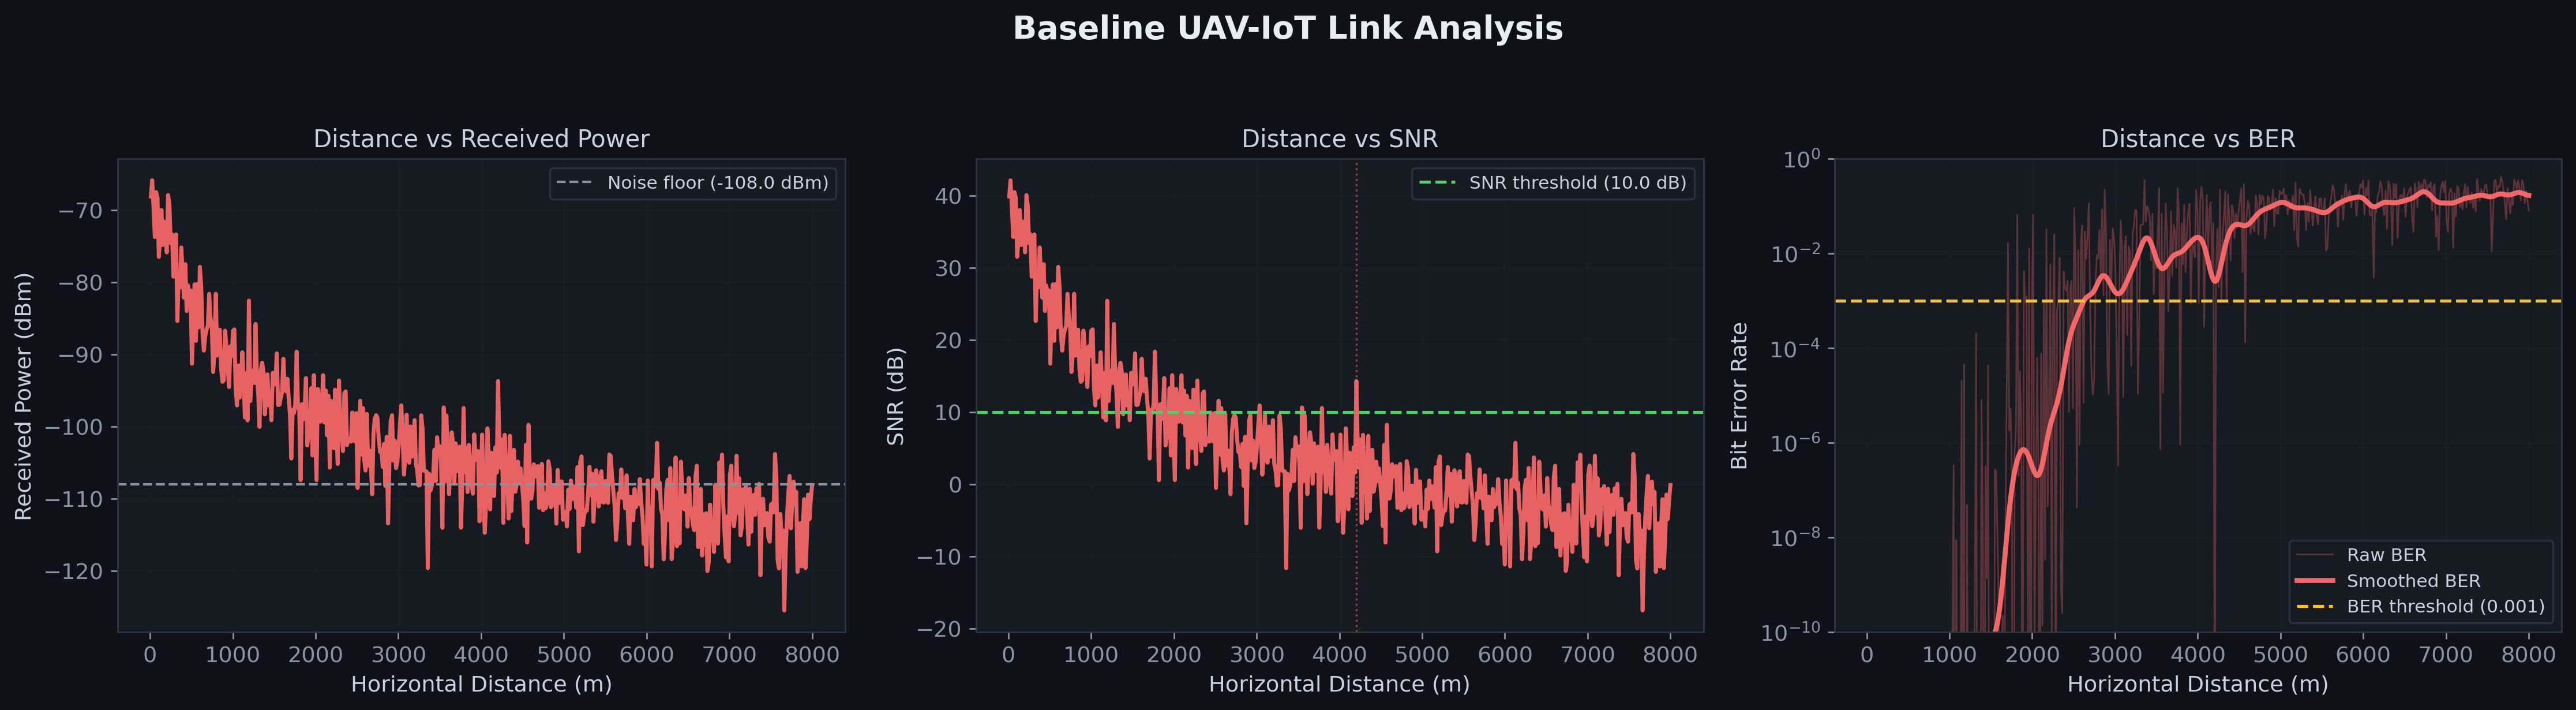
\includegraphics[width=\textwidth]{fig1_baseline_analysis.png}
\caption{\footnotesize Baseline link: SNR drops below 10\,dB at $\sim$2\,km; BER exceeds $10^{-3}$ at \textbf{4,573\,m}.}
\end{figure}
\end{column}

\begin{column}{0.48\textwidth}
\begin{figure}
\centering
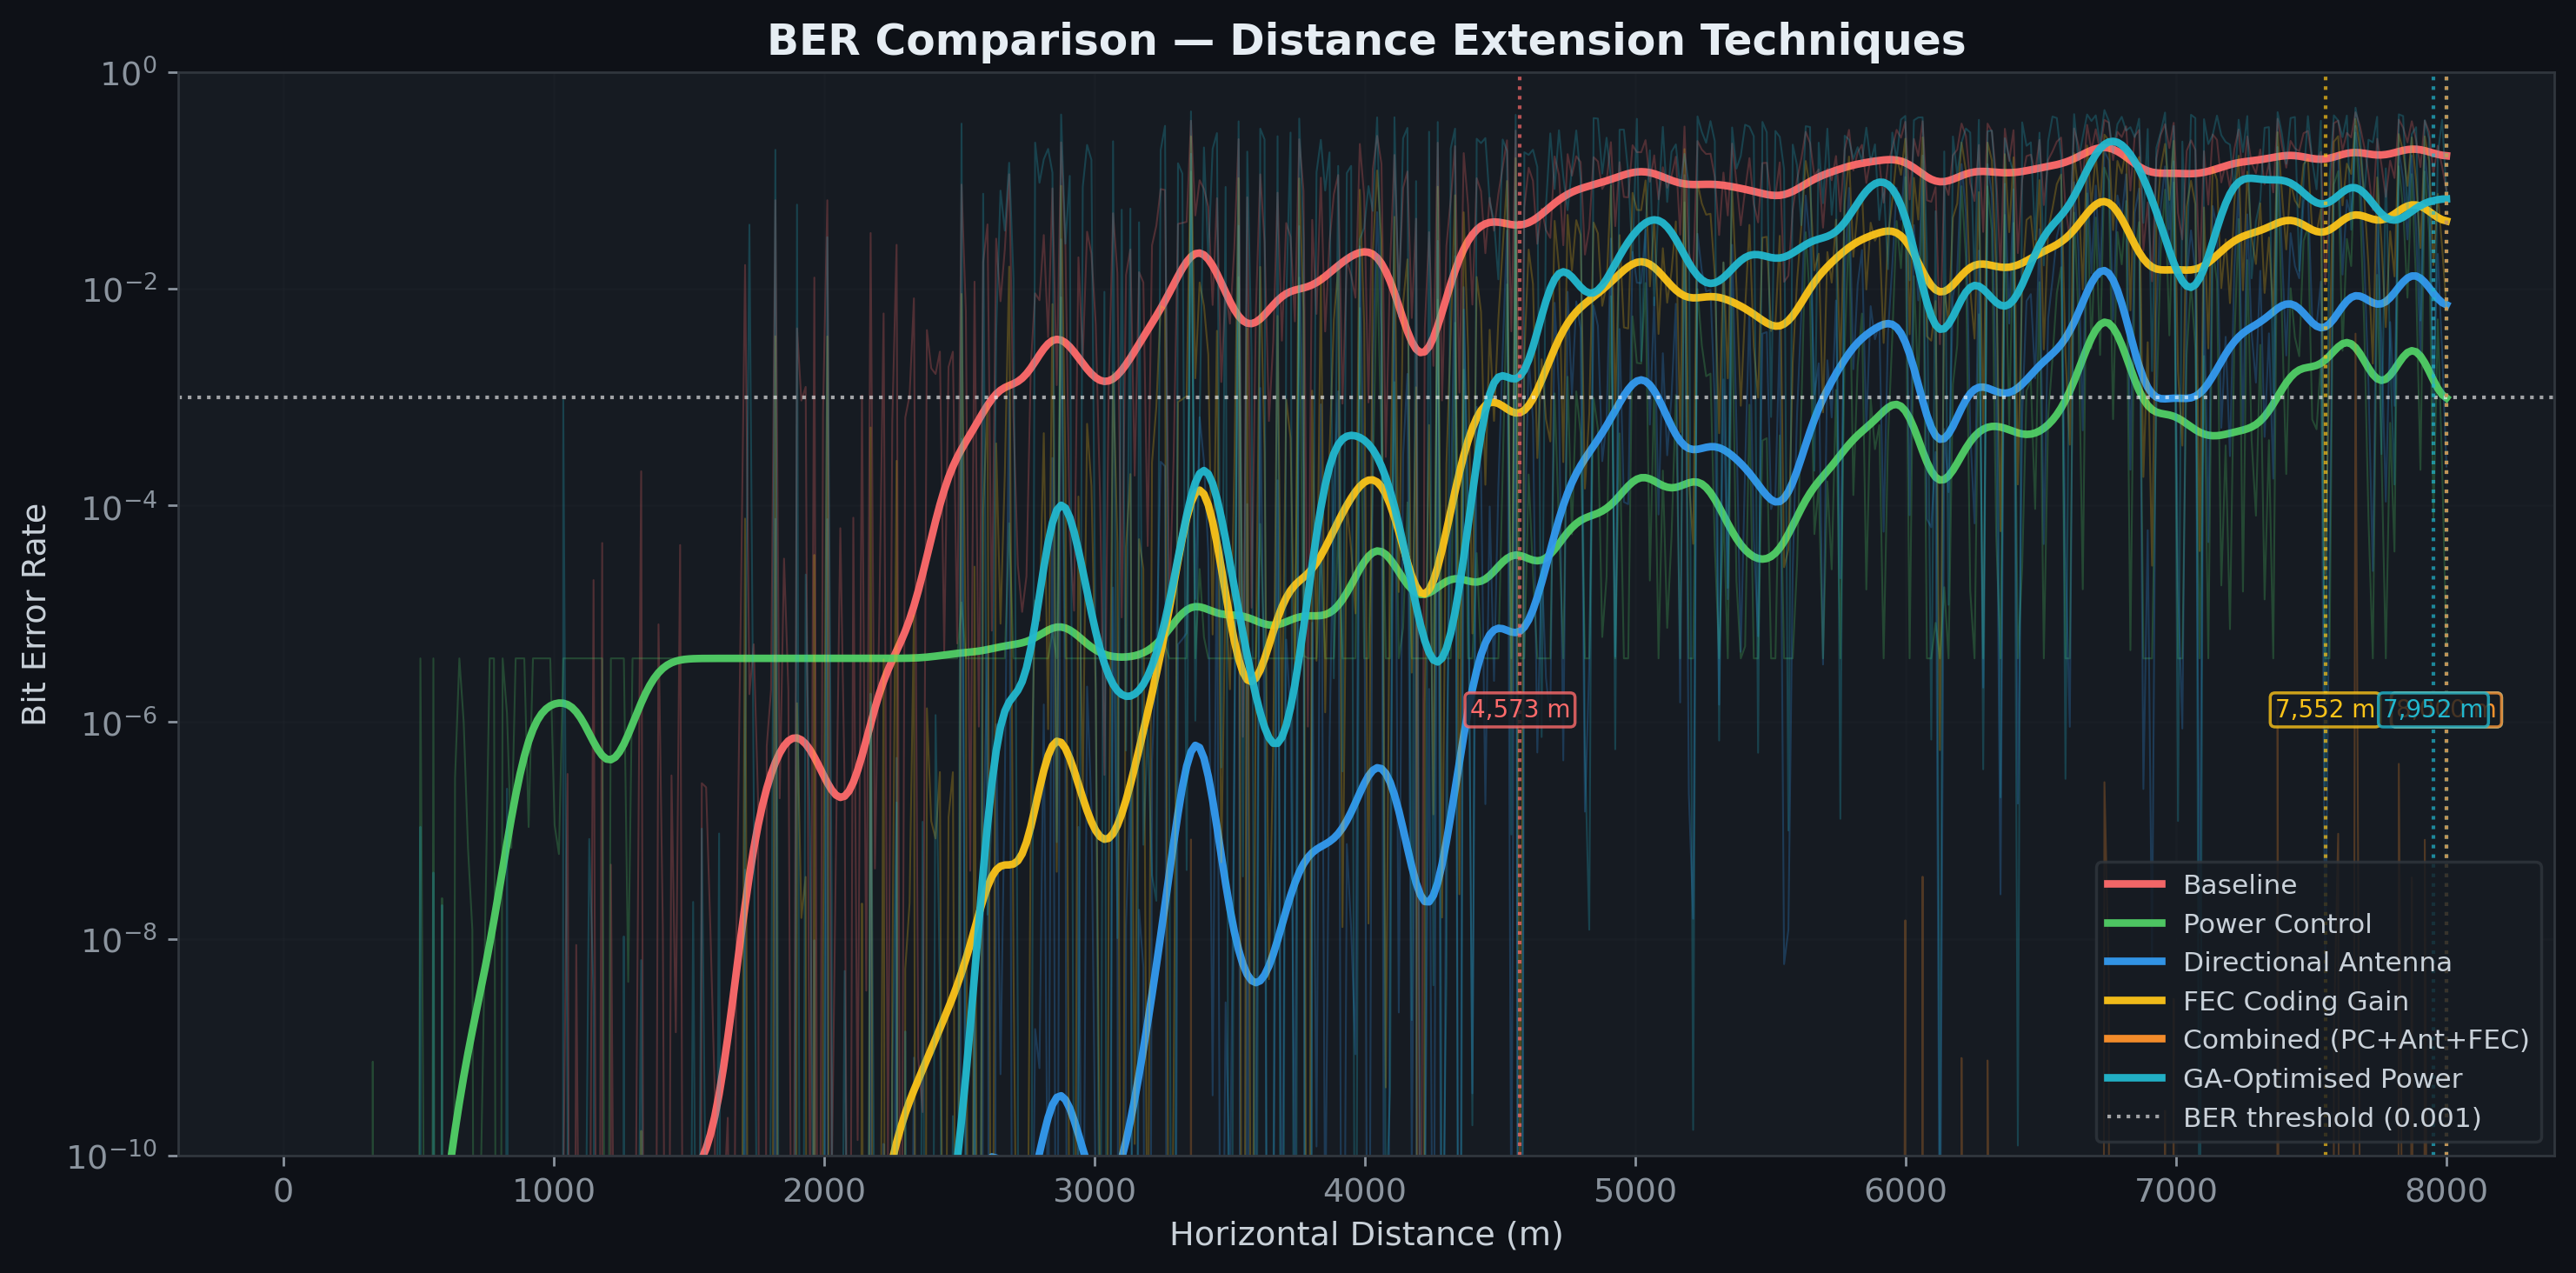
\includegraphics[width=\textwidth]{fig3_ber_comparison.png}
\caption{\footnotesize BER comparison across all techniques with max reliable distance markers.}
\end{figure}
\end{column}

\end{columns}
\end{frame}

% ── Performance Table ────────────────────────────────────────
\begin{frame}{Results — Performance Comparison}
\begin{table}
\centering
\renewcommand{\arraystretch}{1.25}
\begin{tabular}{@{}l r r r r@{}}
\toprule
\textbf{Technique} & \textbf{Range (m)} & \textbf{Impr. (\%)} & \textbf{Power (mW)} & \textbf{EE (m/mW)} \\
\midrule
Baseline (QPSK)       & 4,573 & ---   & 100.0 & 45.7 \\
Power Control          & 8,000 & +74.9 & 560.7 & 14.3 \\
Directional Antenna    & 8,000 & +74.9 & 100.0 & 80.0 \\
FEC Coding             & 7,552 & +65.1 & 100.0 & 75.5 \\
Combined               & 8,000 & +74.9 & 560.7 & 14.3 \\
\rowcolor{accentcyan!15}
\textbf{GA-Optimised}  & \textbf{7,952} & \textbf{+73.9} & \textbf{248.1} & \textbf{32.1} \\
\bottomrule
\end{tabular}
\end{table}

\vspace{0.3cm}
\begin{alertblock}{Key Finding}
GA achieves \textbf{99.4\%} of maximum range with \textbf{55.7\% less power} than threshold-based control (248.1\,mW vs.\ 560.7\,mW), yielding \textbf{32.1\,m/mW} energy efficiency.
\end{alertblock}
\end{frame}

% ── GA & Energy ──────────────────────────────────────────────
\begin{frame}{Results — GA Convergence \& Energy Analysis}
\begin{columns}[T]

\begin{column}{0.48\textwidth}
\begin{figure}
\centering
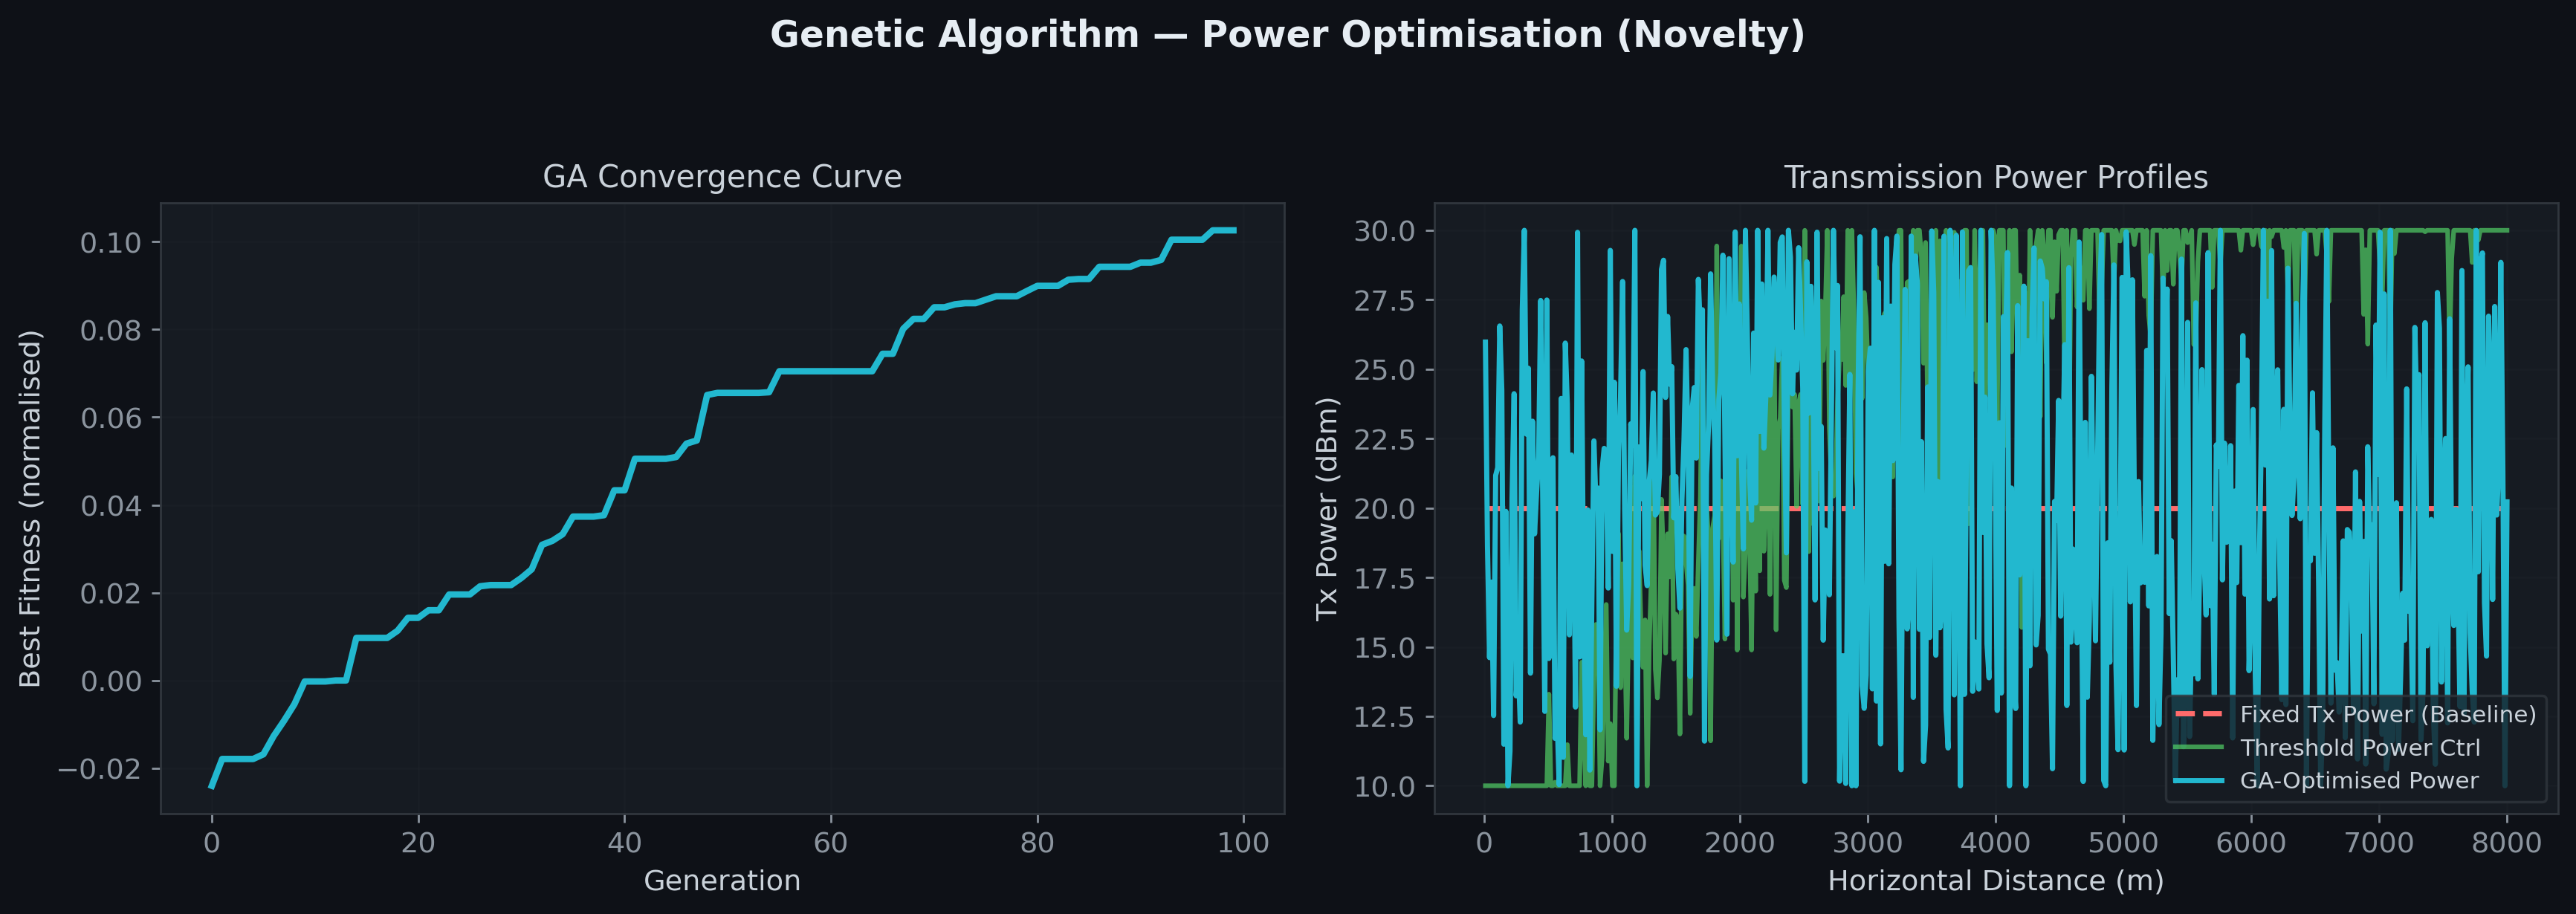
\includegraphics[width=\textwidth]{fig5_ga_optimization.png}
\caption{\footnotesize GA convergence and optimised Tx power profile. Low power at short range; selective increase at link-budget limits.}
\end{figure}
\end{column}

\begin{column}{0.48\textwidth}
\begin{figure}
\centering
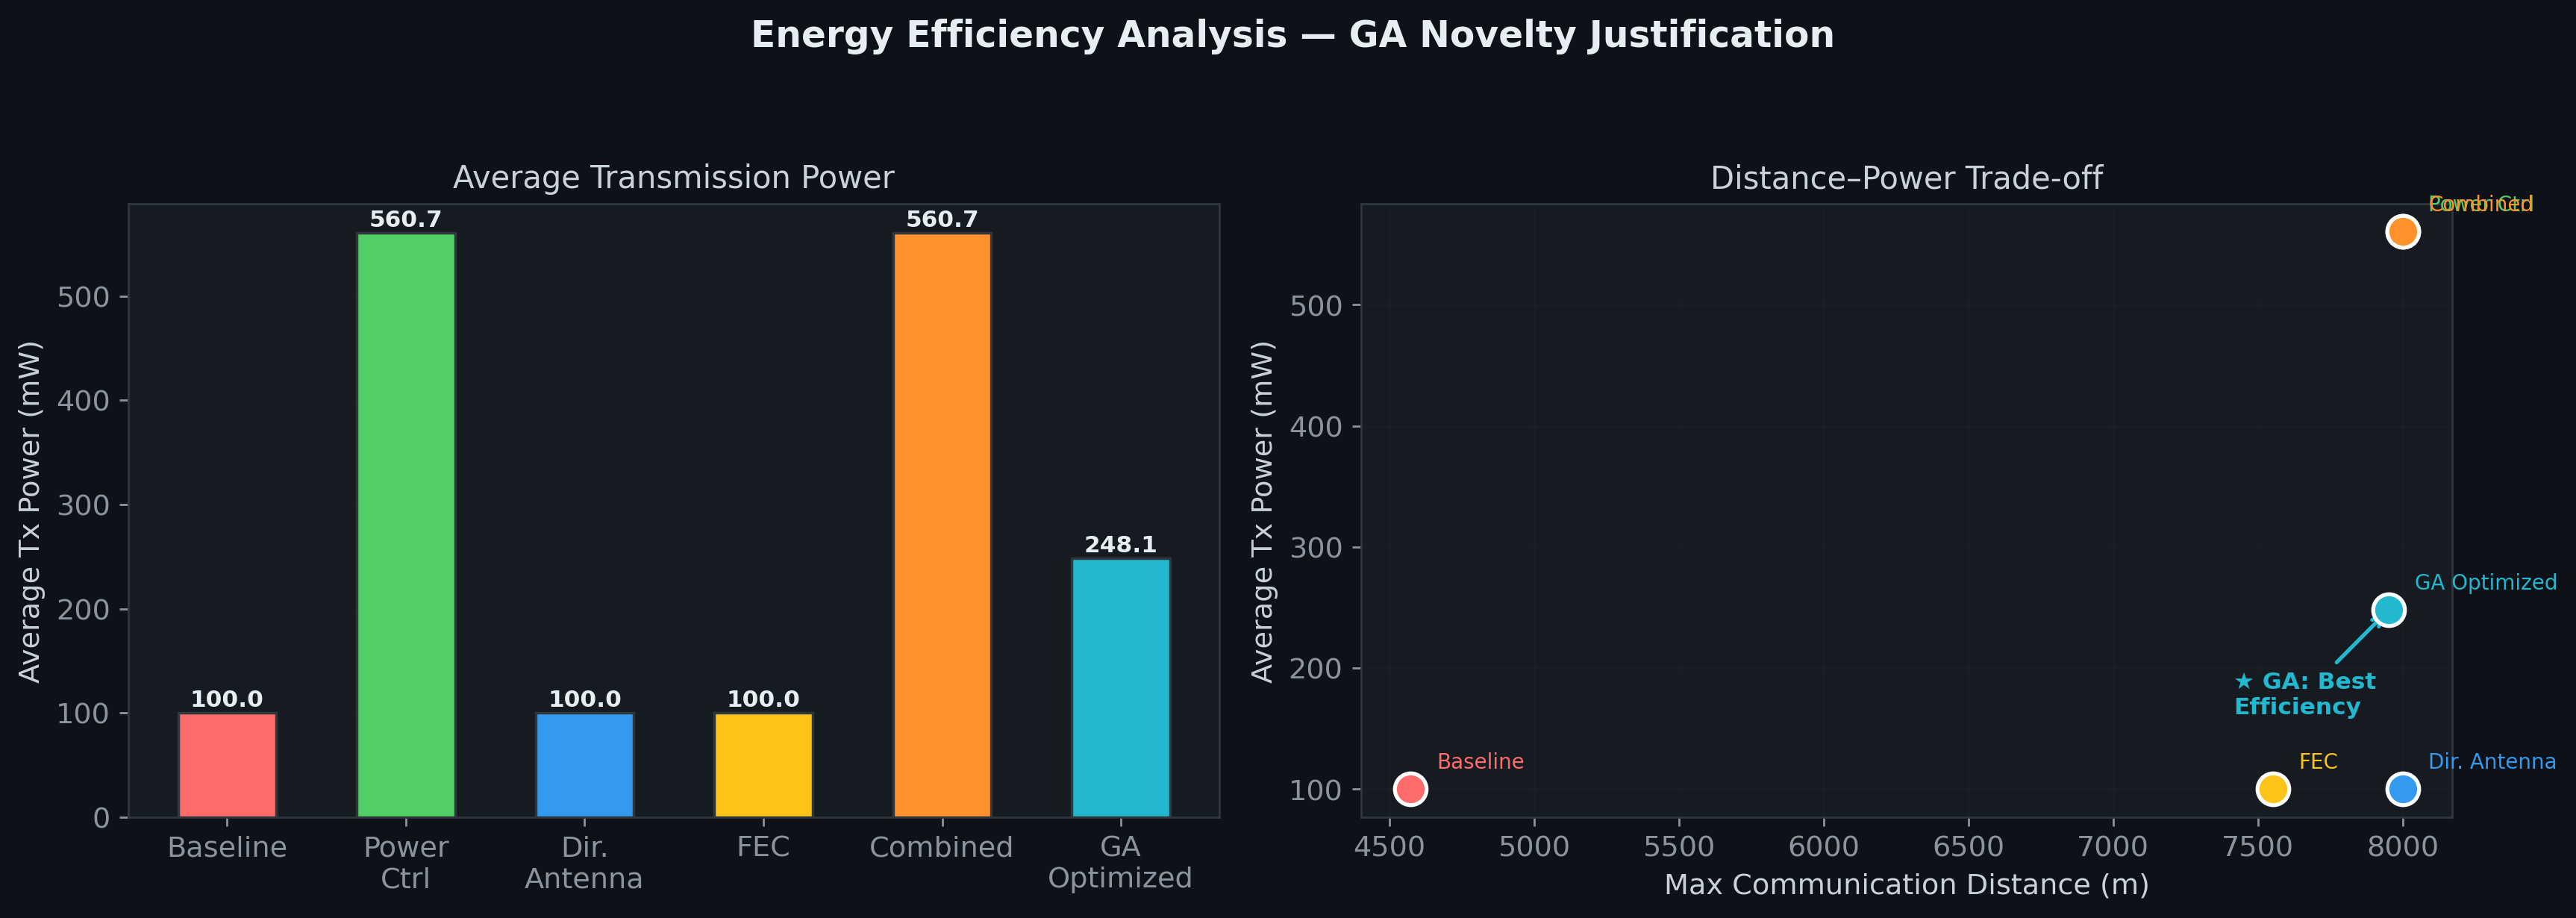
\includegraphics[width=\textwidth]{fig8_energy_analysis.png}
\caption{\footnotesize Energy analysis: average power, formal EE (m/mW), and distance--power trade-off.}
\end{figure}
\end{column}

\end{columns}
\end{frame}

% ── Fading & Altitude ────────────────────────────────────────
\begin{frame}{Results — Fading Channels \& Altitude Analysis}
\begin{columns}[T]

\begin{column}{0.48\textwidth}
\begin{figure}
\centering
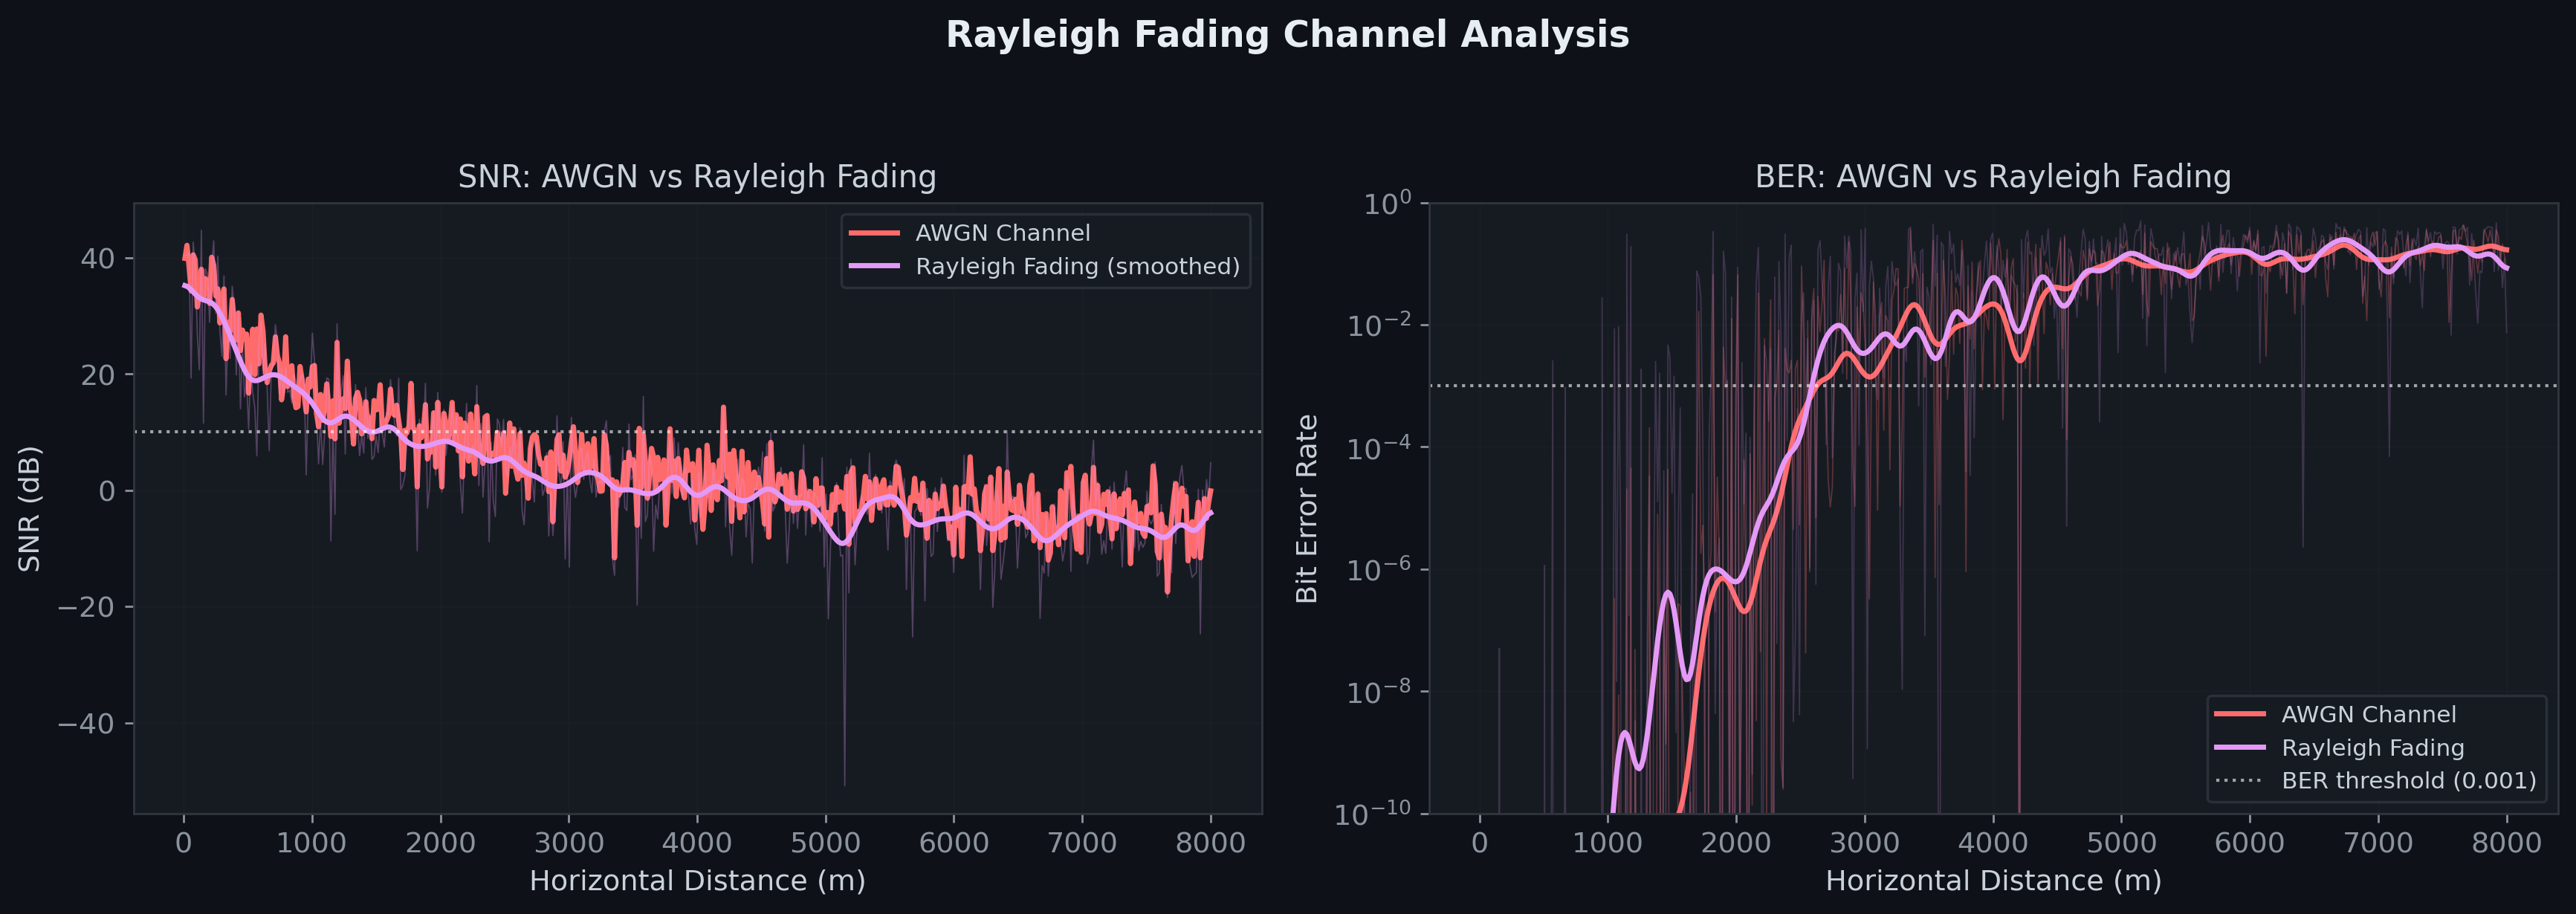
\includegraphics[width=\textwidth]{fig10_rayleigh_fading.png}
\caption{\footnotesize AWGN vs Rayleigh vs Rician ($K\!=\!6$). Rician closely tracks AWGN baseline.}
\end{figure}
\end{column}

\begin{column}{0.48\textwidth}
\begin{block}{Altitude Trade-off}
\renewcommand{\arraystretch}{1.25}
\centering
\begin{tabular}{@{}c c c c@{}}
\toprule
\textbf{Alt. (m)} & \textbf{PL Exp.} & \textbf{Range (m)} & \textbf{vs 100\,m} \\
\midrule
50  & 3.0 & 1,195  & $0.26\times$ \\
100 & 2.5 & 4,573  & ref. \\
200 & 2.2 & 8,000  & $1.75\times$ \\
\bottomrule
\end{tabular}
\end{block}

\vspace{0.3cm}
\begin{exampleblock}{Insight}
Higher altitude $\Rightarrow$ better LoS $\Rightarrow$ lower path-loss exponent $\Rightarrow$ \textbf{6.7$\times$} range improvement from 50\,m to 200\,m.
\end{exampleblock}
\end{column}

\end{columns}
\end{frame}

% ── SNR & Rx Power ───────────────────────────────────────────
\begin{frame}{Results --- SNR \& Received Power Comparison}
\begin{columns}[T]
\begin{column}{0.48\textwidth}
\begin{figure}
\centering
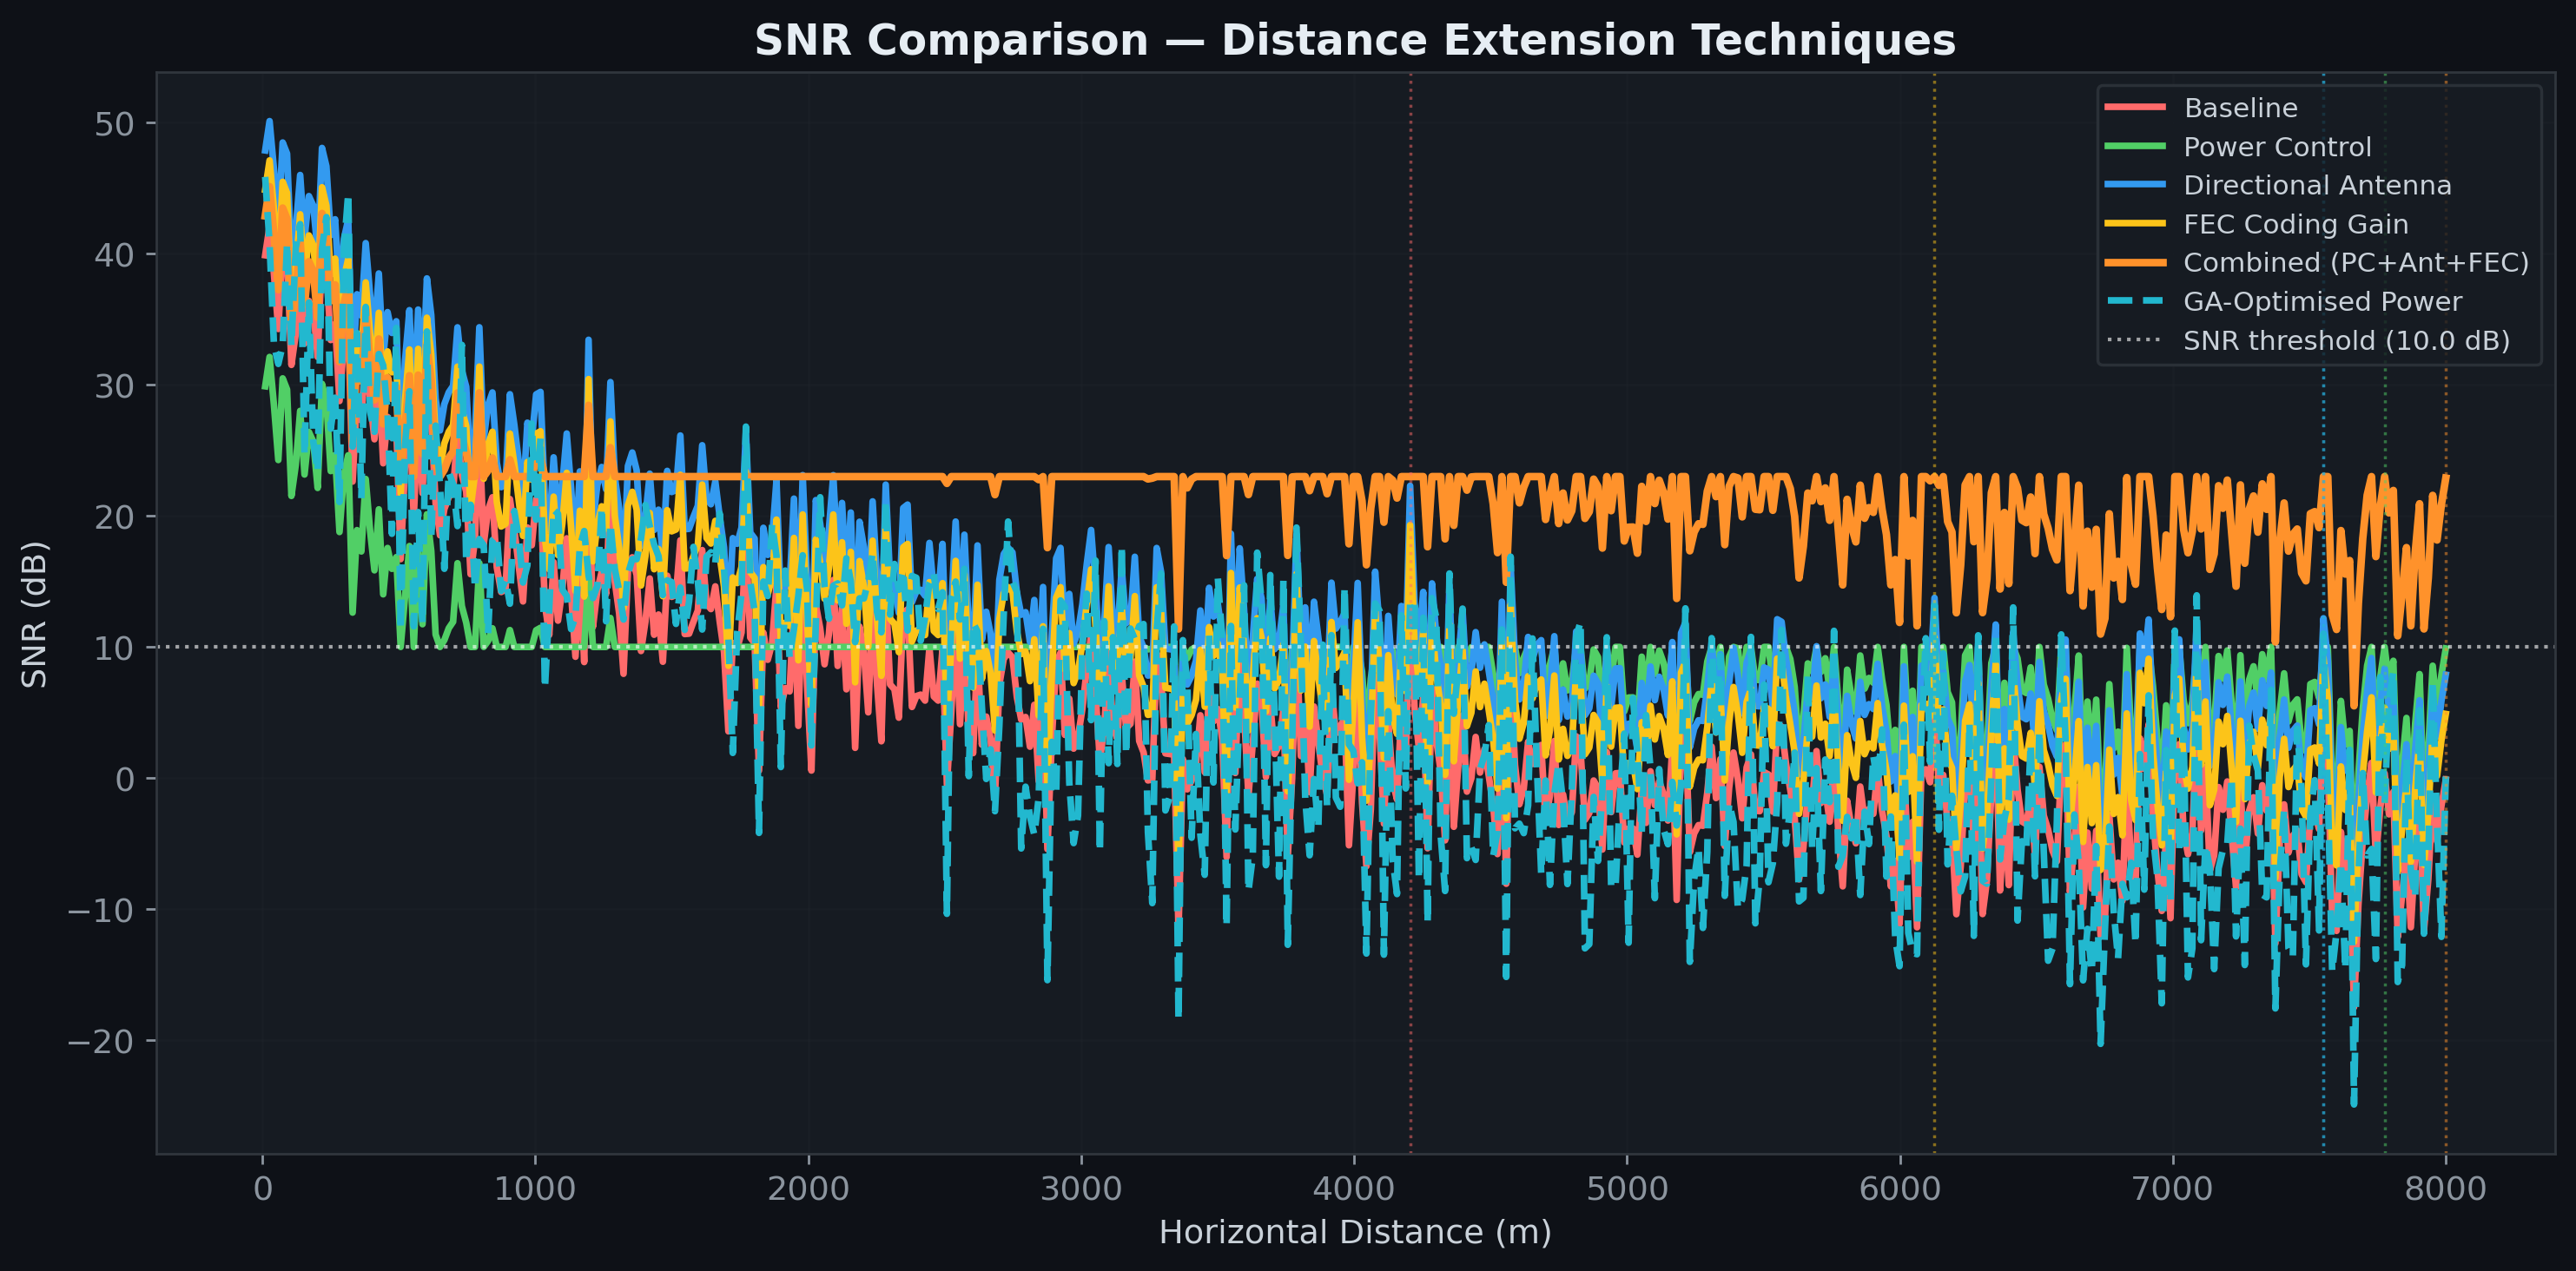
\includegraphics[width=\textwidth]{fig2_snr_comparison.png}
\caption{\footnotesize SNR vs.\ distance for all techniques. Power control and combined maintain SNR above threshold longest.}
\end{figure}
\end{column}
\begin{column}{0.48\textwidth}
\begin{figure}
\centering
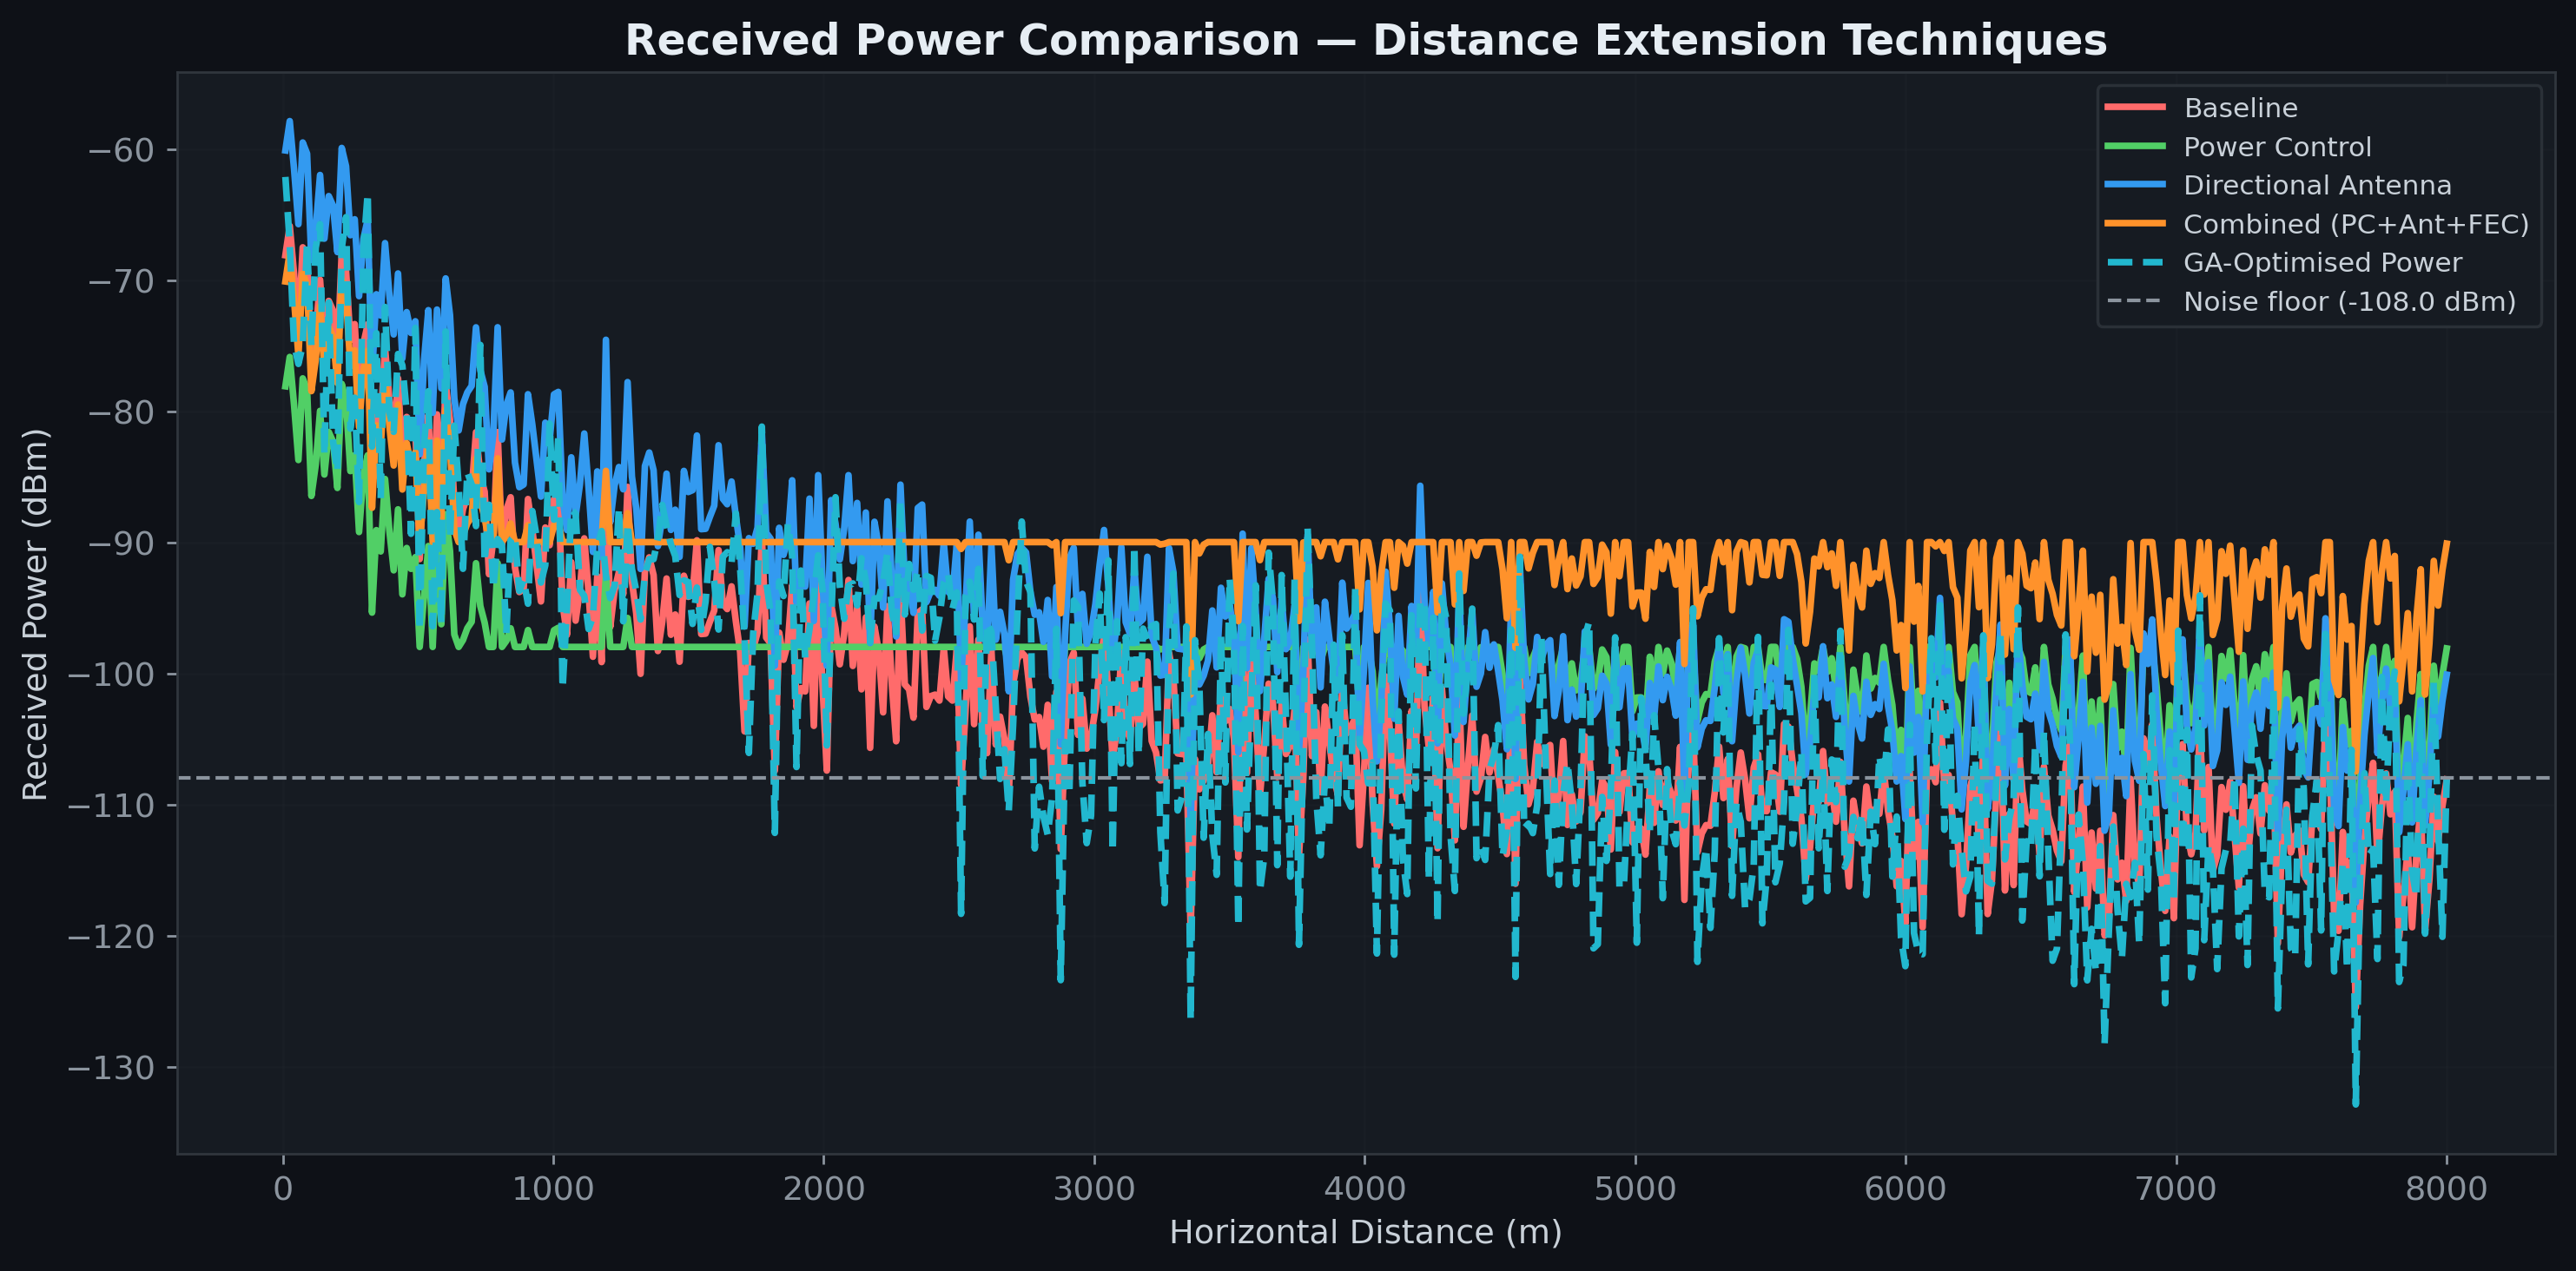
\includegraphics[width=\textwidth]{fig4_rx_power_comparison.png}
\caption{\footnotesize Received power comparison. Directional antenna provides +8\,dB constant gain across all distances.}
\end{figure}
\end{column}
\end{columns}
\end{frame}

% ── Throughput Analysis ──────────────────────────────────────
\begin{frame}{Results --- Throughput \& Adaptive Modulation}
\begin{columns}[T]
\begin{column}{0.48\textwidth}
\begin{figure}
\centering
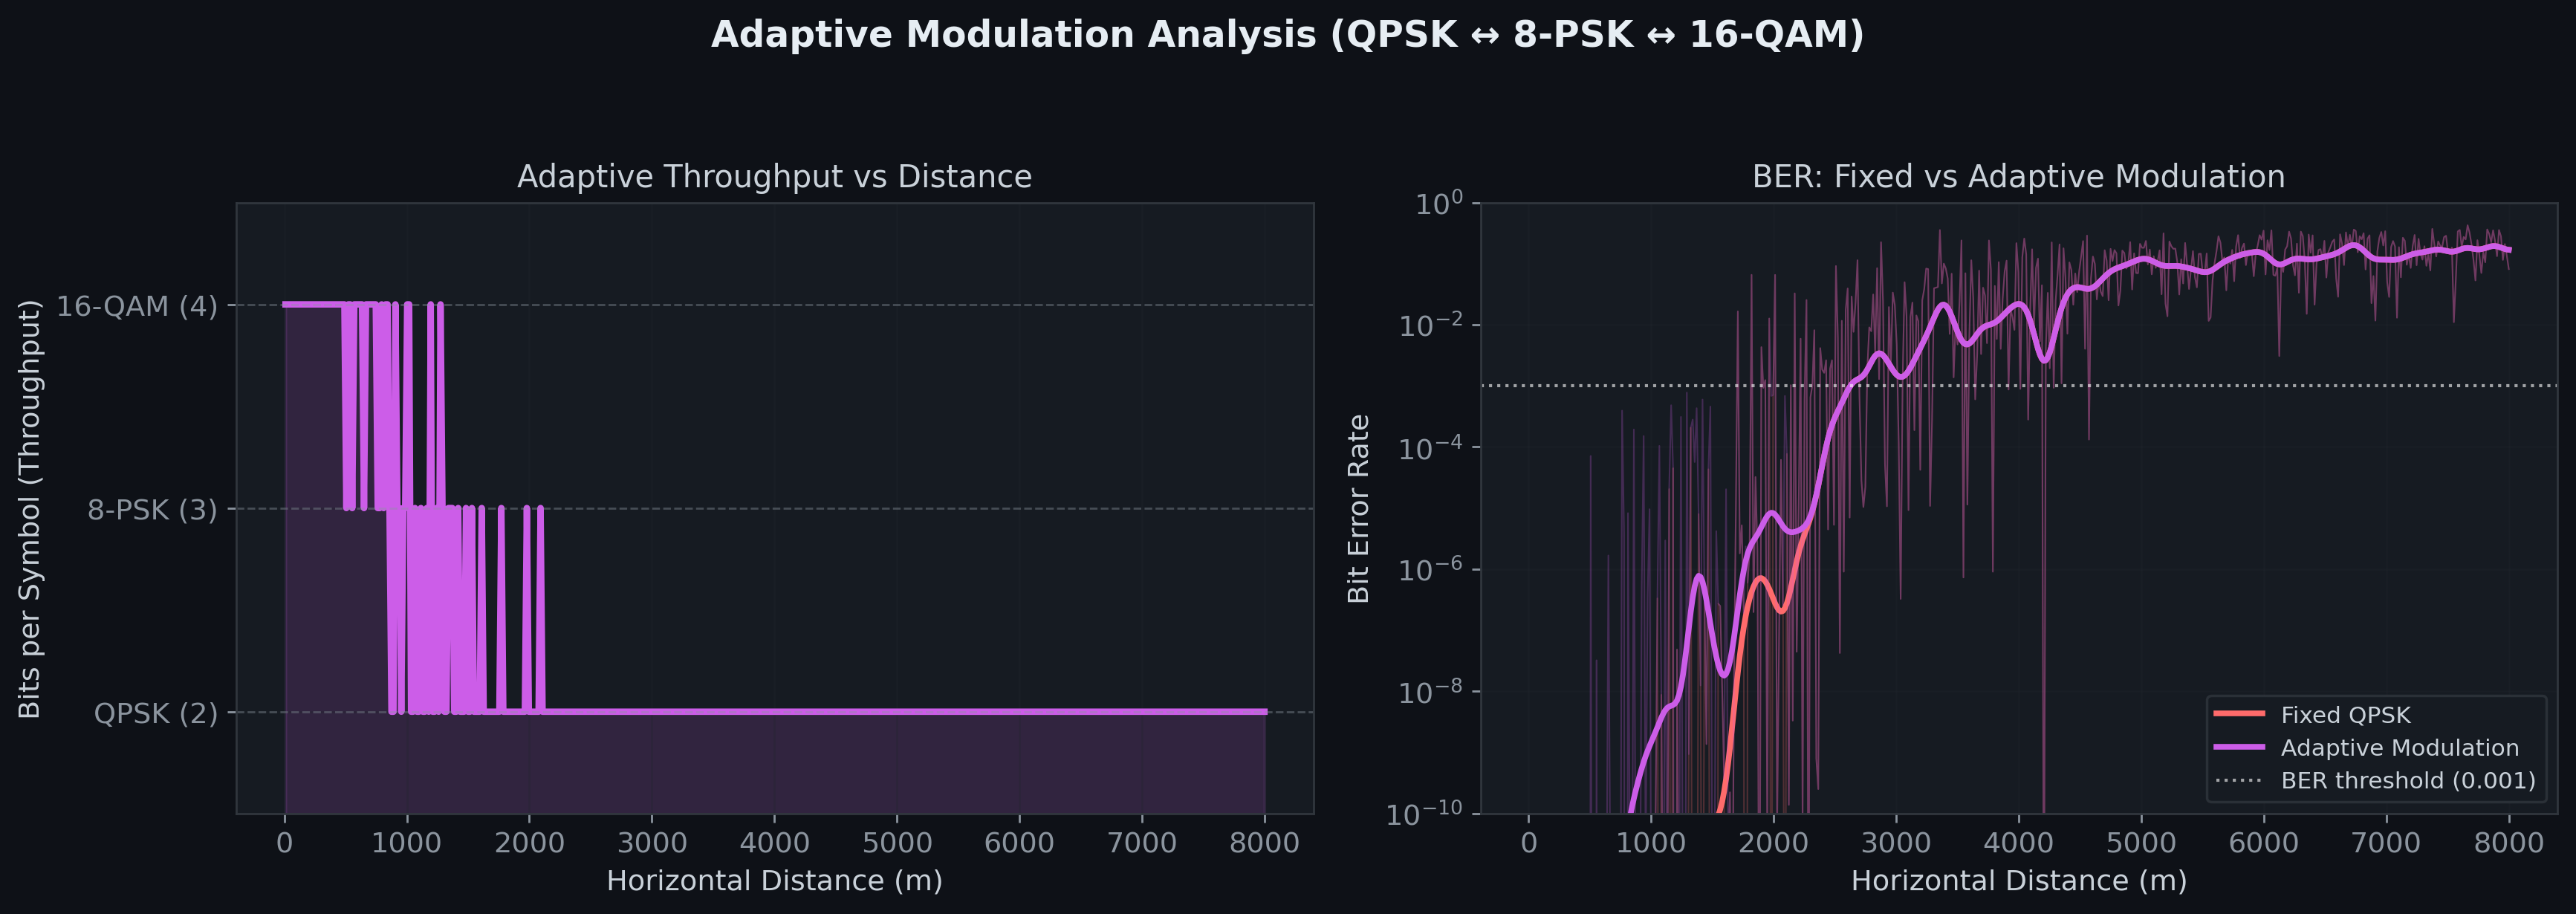
\includegraphics[width=\textwidth]{fig6_adaptive_modulation.png}
\caption{\footnotesize Adaptive modulation transitions: 16-QAM $\to$ 8-PSK $\to$ QPSK as distance increases.}
\end{figure}
\end{column}
\begin{column}{0.48\textwidth}
\begin{figure}
\centering
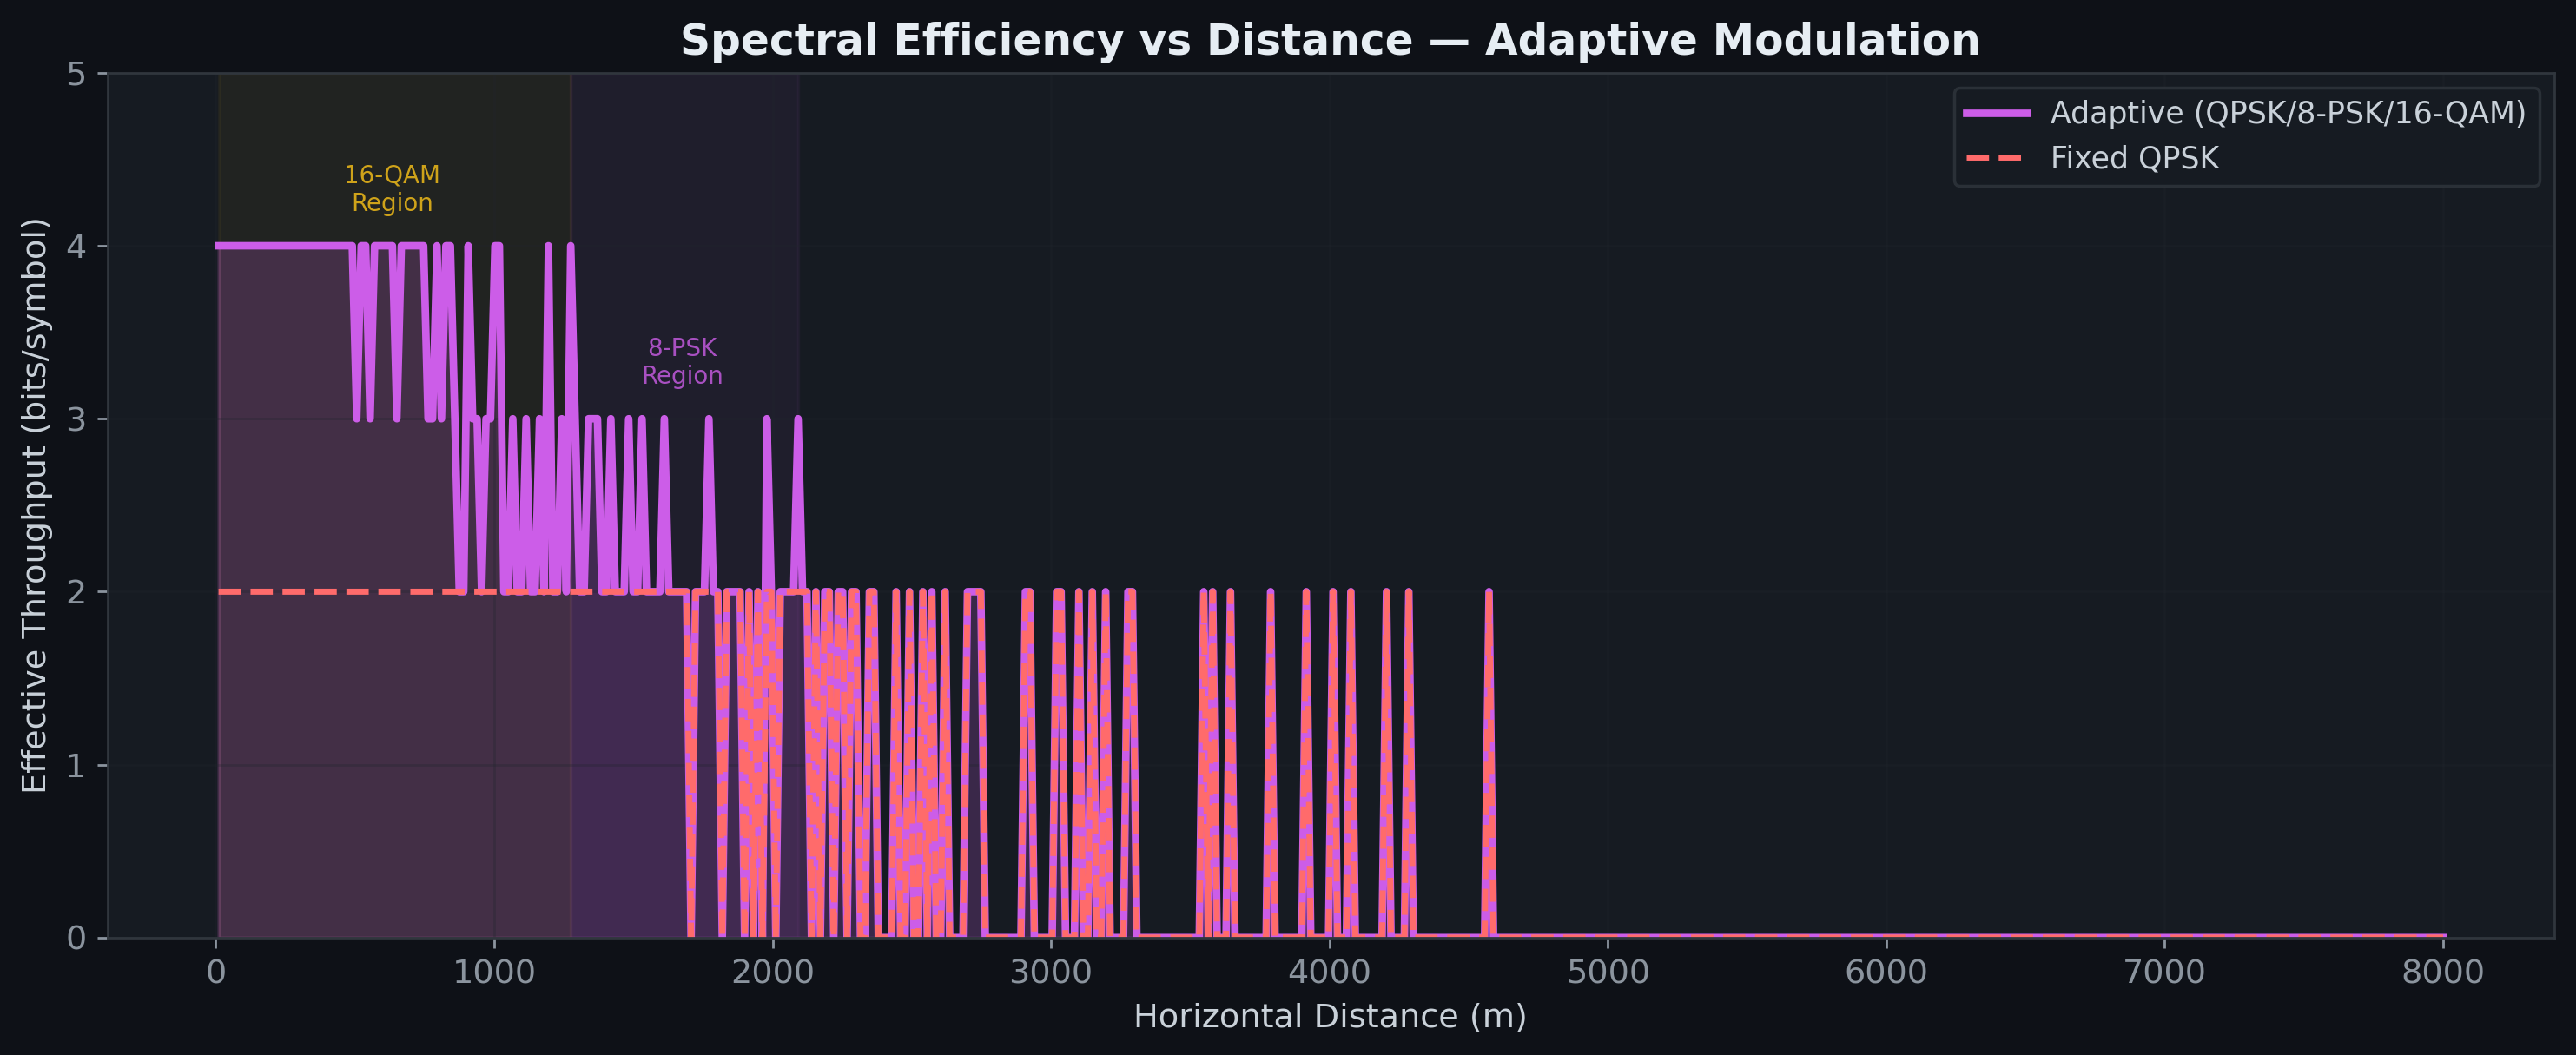
\includegraphics[width=\textwidth]{fig11_throughput_analysis.png}
\caption{\footnotesize Throughput analysis under three-tier adaptive modulation scheme.}
\end{figure}
\end{column}
\end{columns}
\vspace{0.2cm}
\begin{exampleblock}{Throughput Insight}
Adaptive modulation provides \textbf{4\,bps/Hz} (16-QAM) at short range, transitioning to \textbf{2\,bps/Hz} (QPSK) at extended range --- \textbf{33\% higher near-field throughput} than fixed QPSK.
\end{exampleblock}
\end{frame}

% ── Summary Dashboard ────────────────────────────────────────
\begin{frame}{Results --- Summary Dashboard}
\begin{figure}
\centering
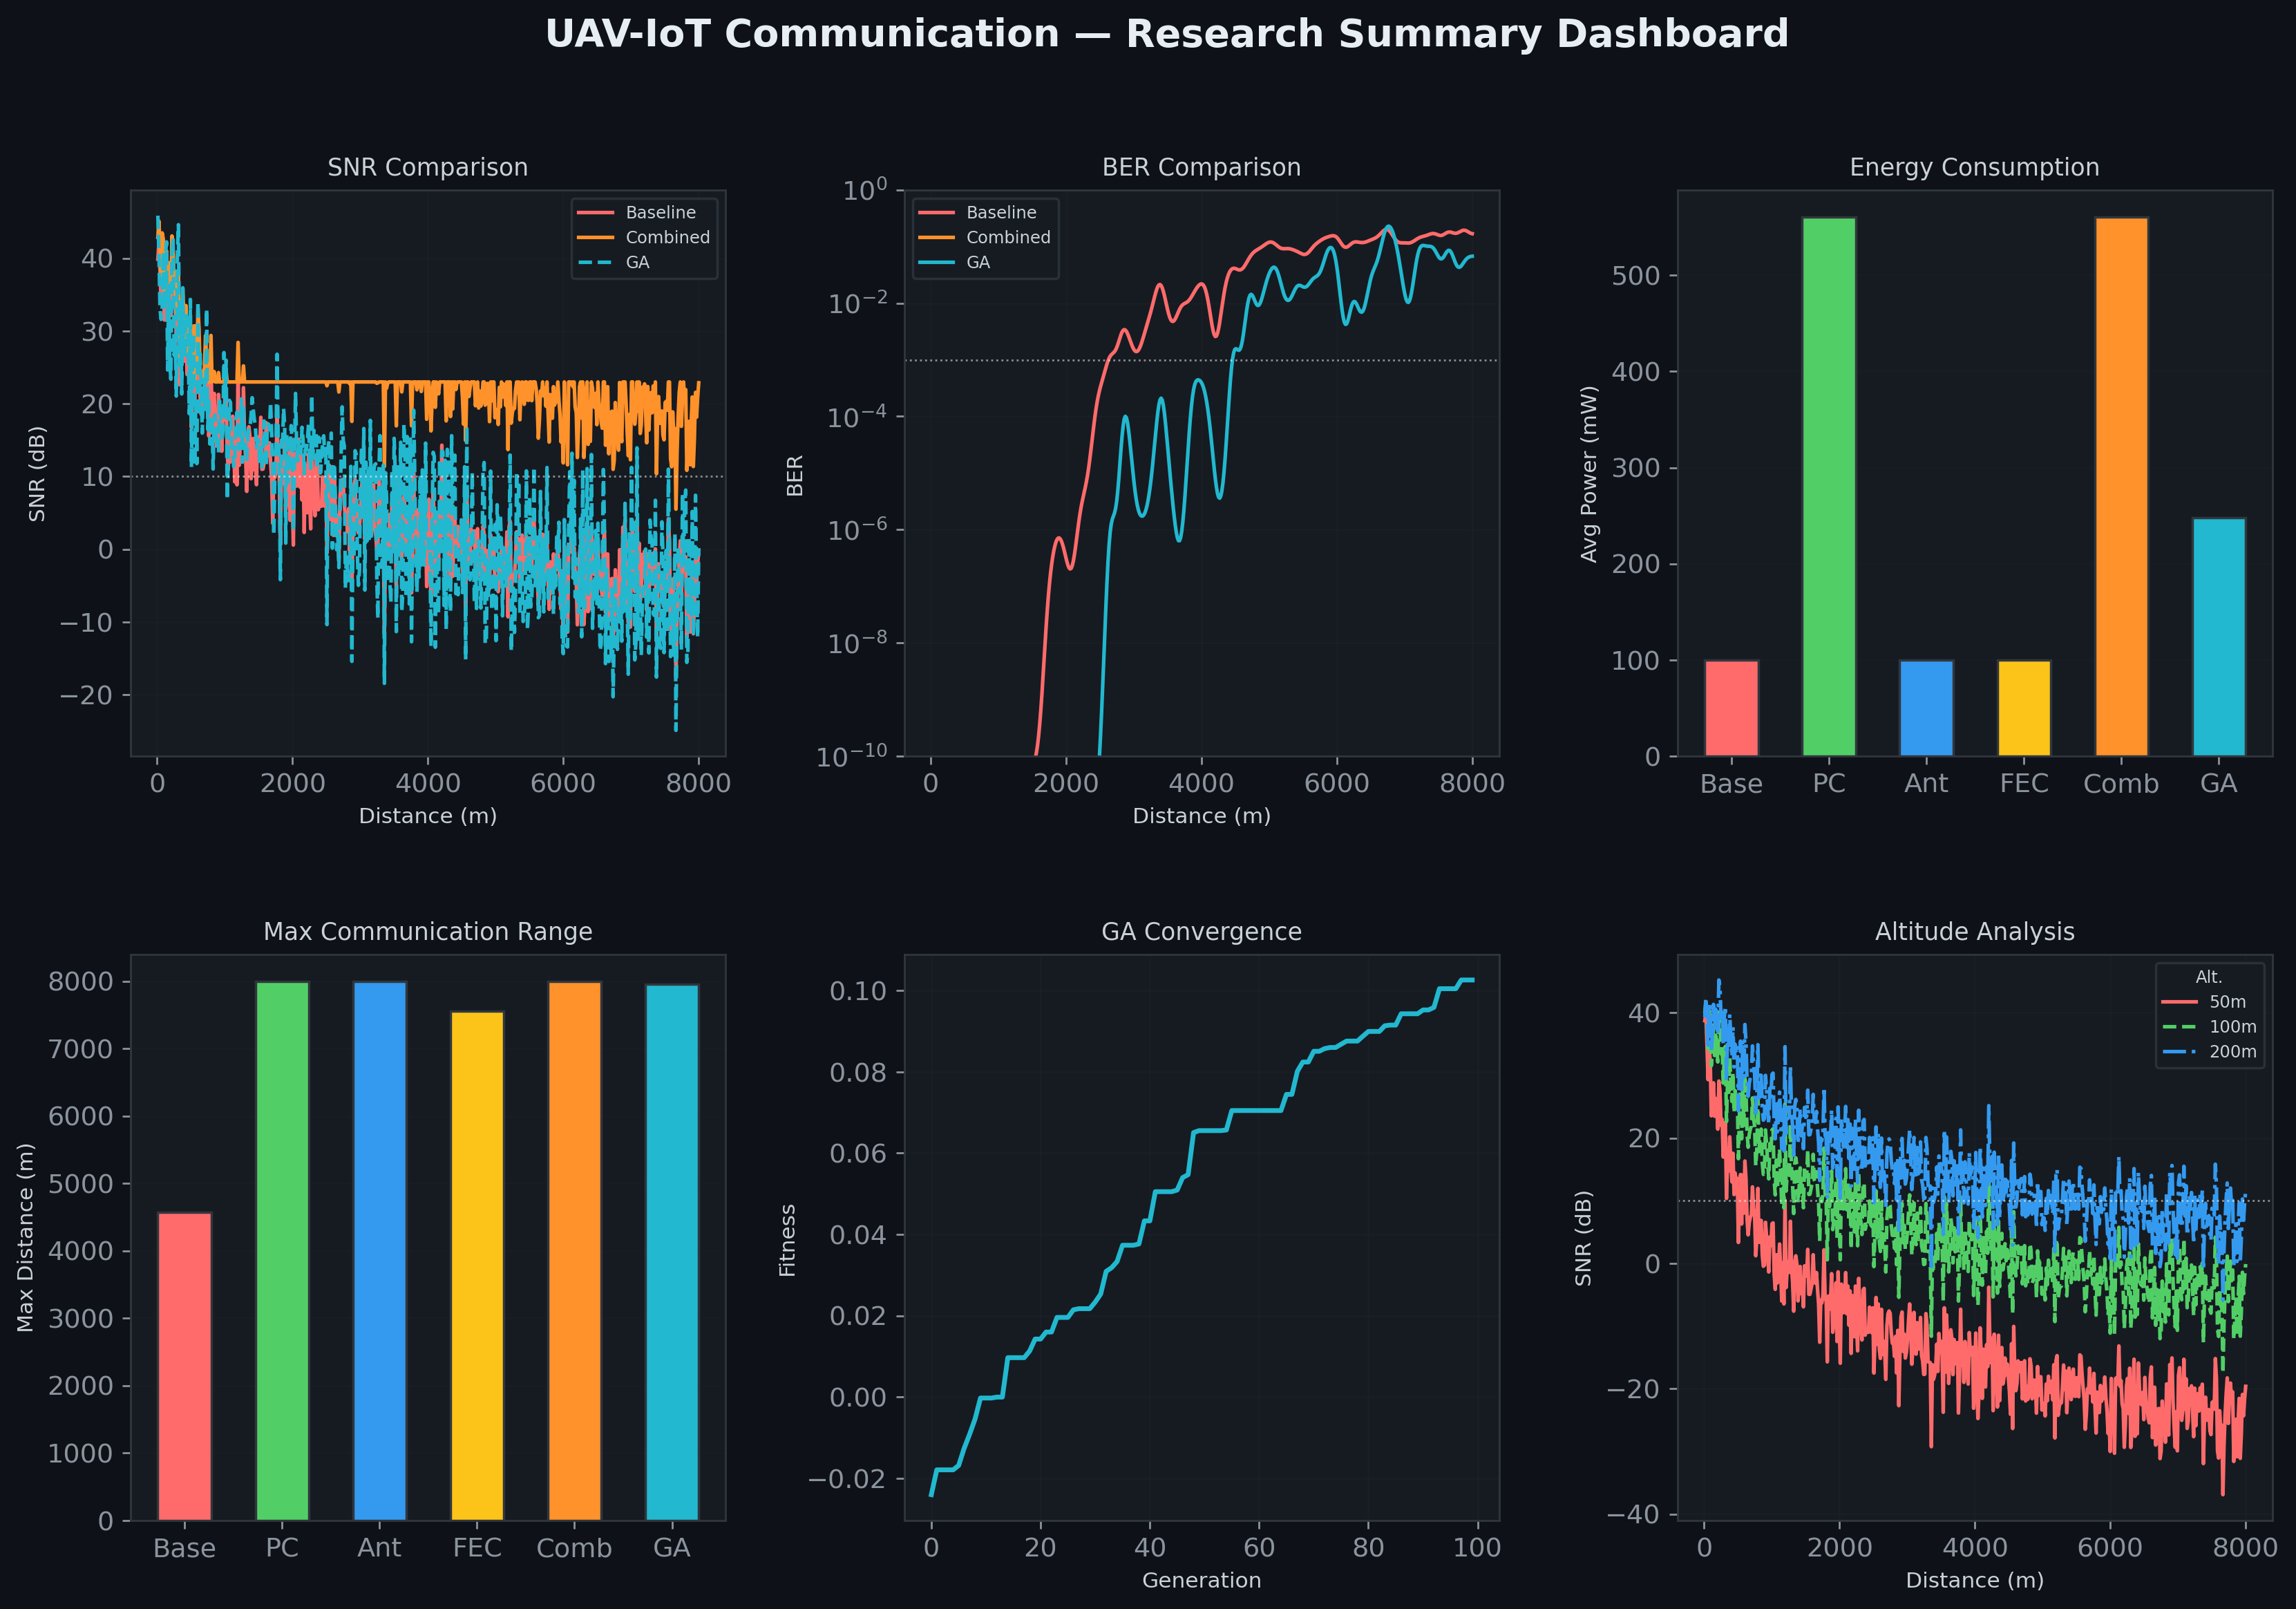
\includegraphics[width=0.82\textwidth]{fig12_summary_dashboard.png}
\caption{Enhanced $3\!\times\!3$ summary dashboard consolidating all research results.}
\end{figure}
\end{frame}

% ── Distance Summary ─────────────────────────────────────────
\begin{frame}{Results --- Max Distance Summary}
\begin{columns}[T]
\begin{column}{0.48\textwidth}
\begin{figure}
\centering
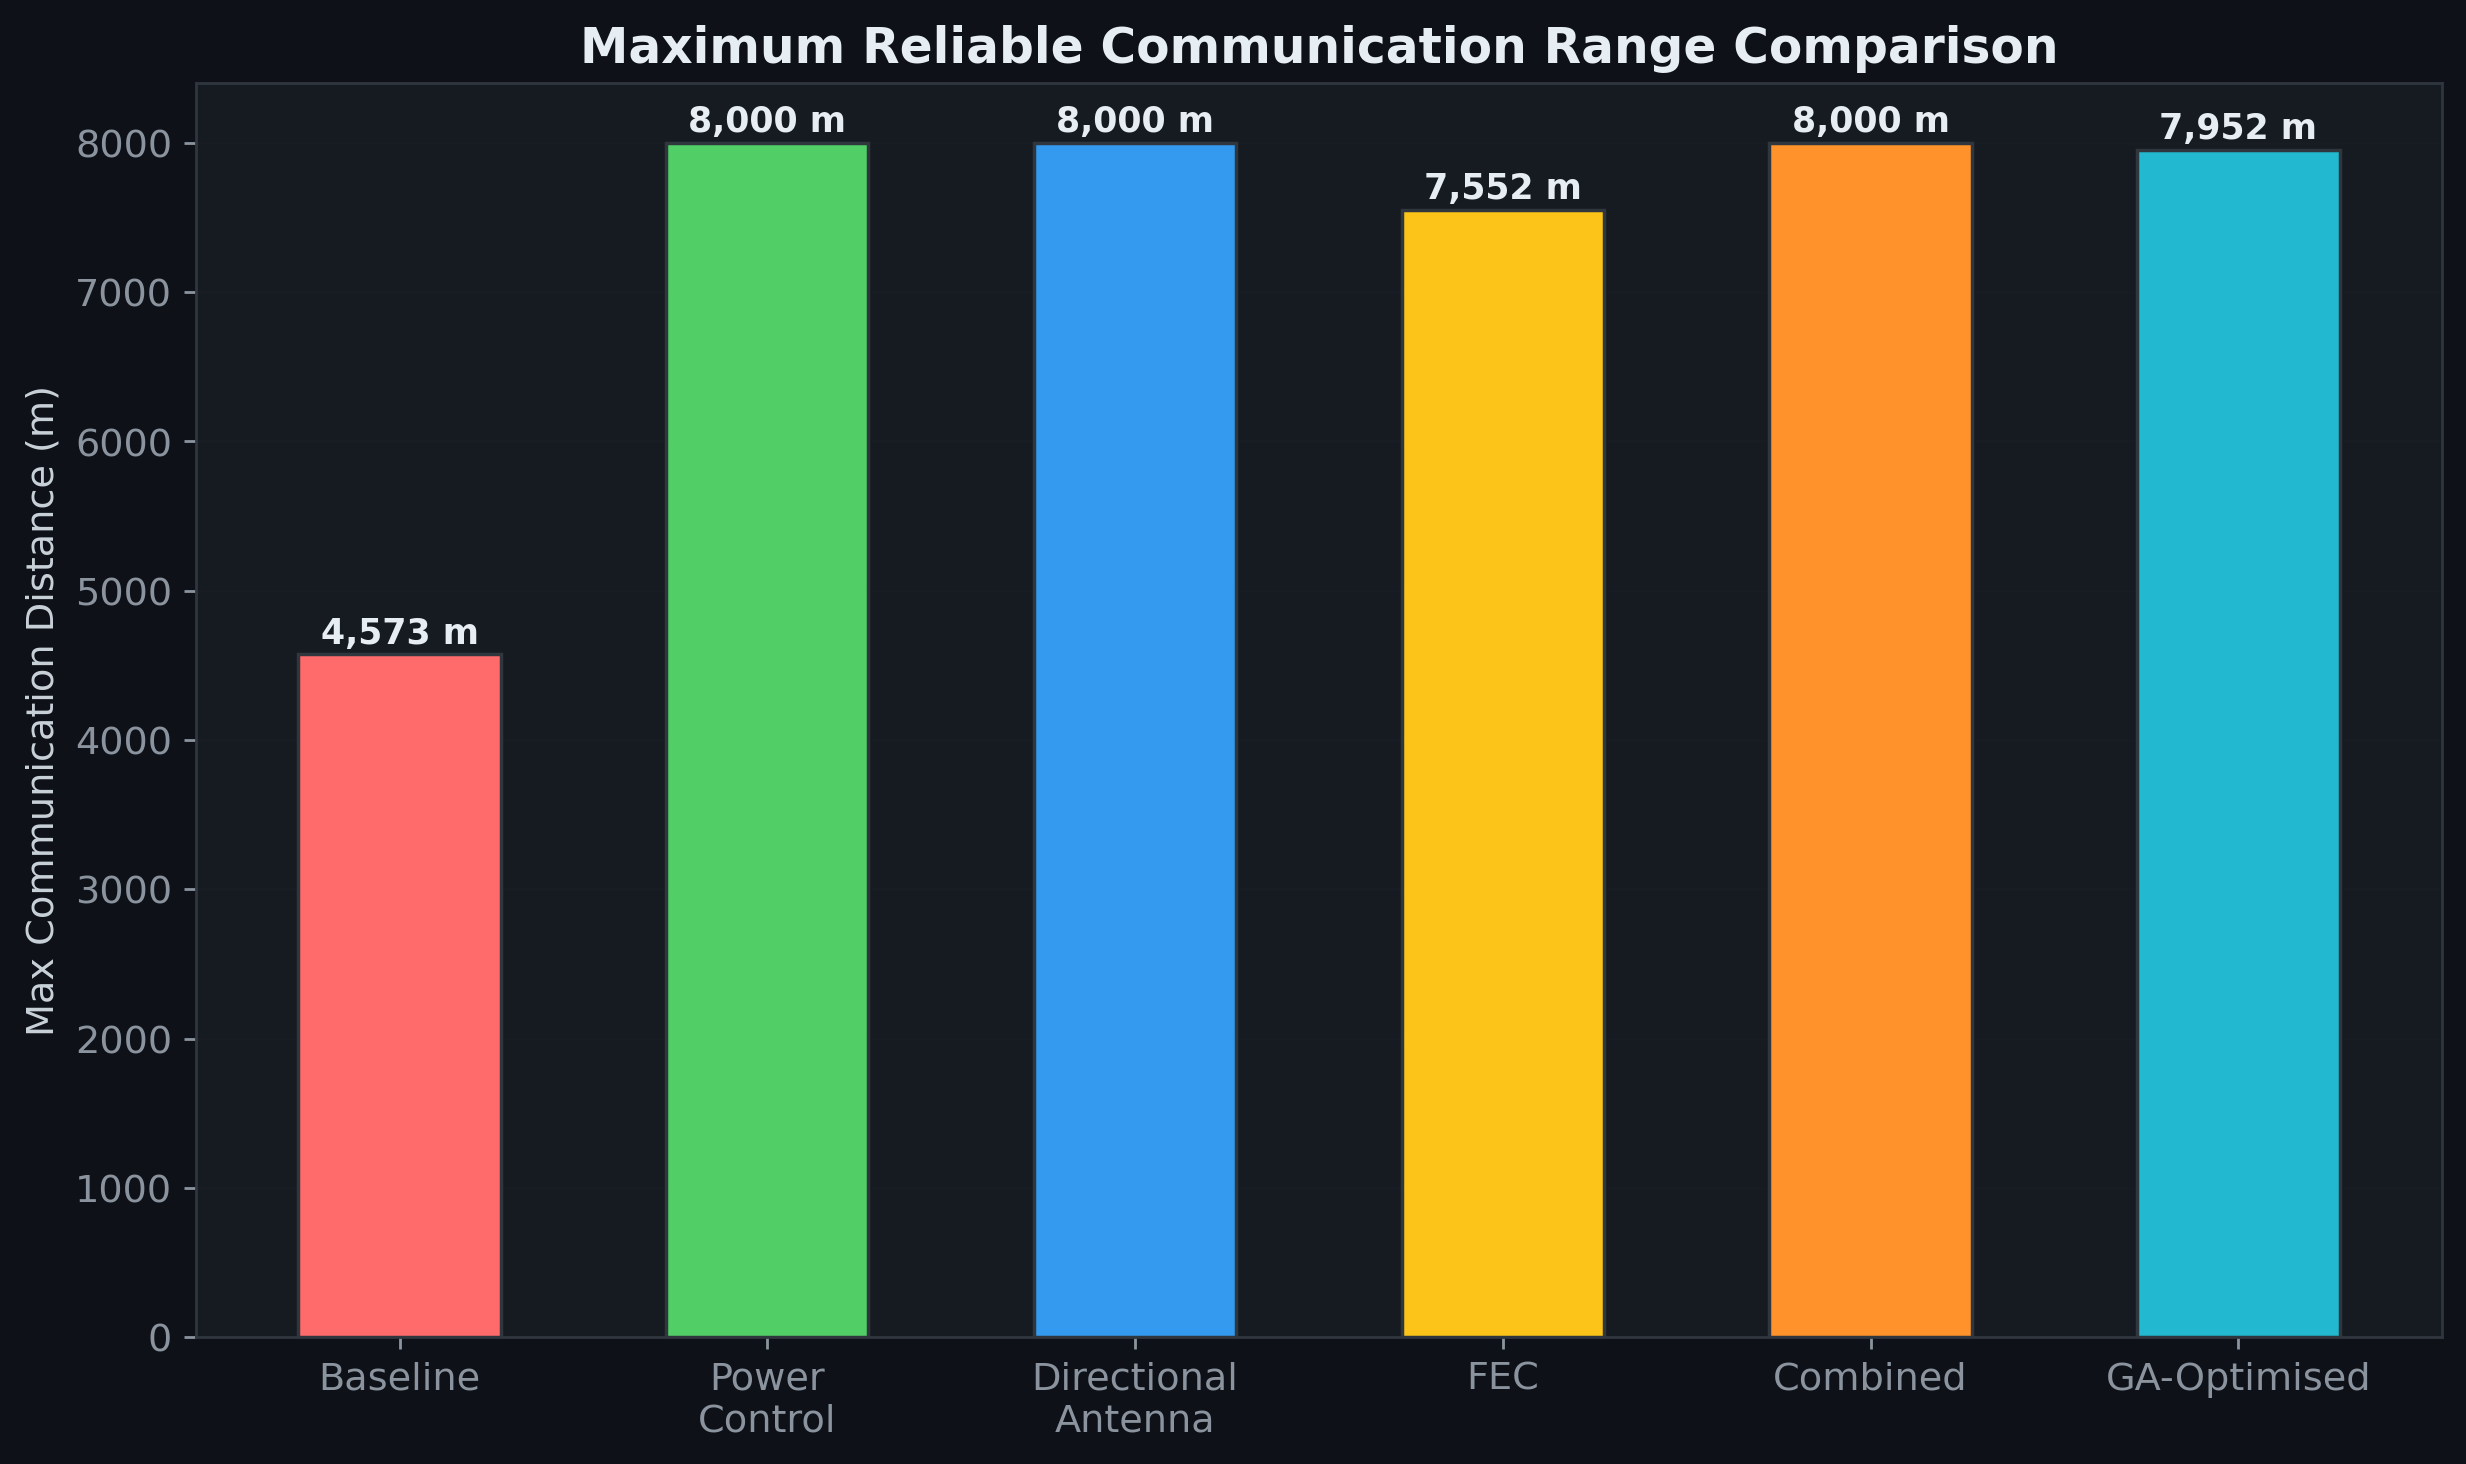
\includegraphics[width=\textwidth]{fig7_distance_summary.png}
\caption{\footnotesize Maximum reliable distance achieved by each technique.}
\end{figure}
\end{column}
\begin{column}{0.48\textwidth}
\begin{figure}
\centering
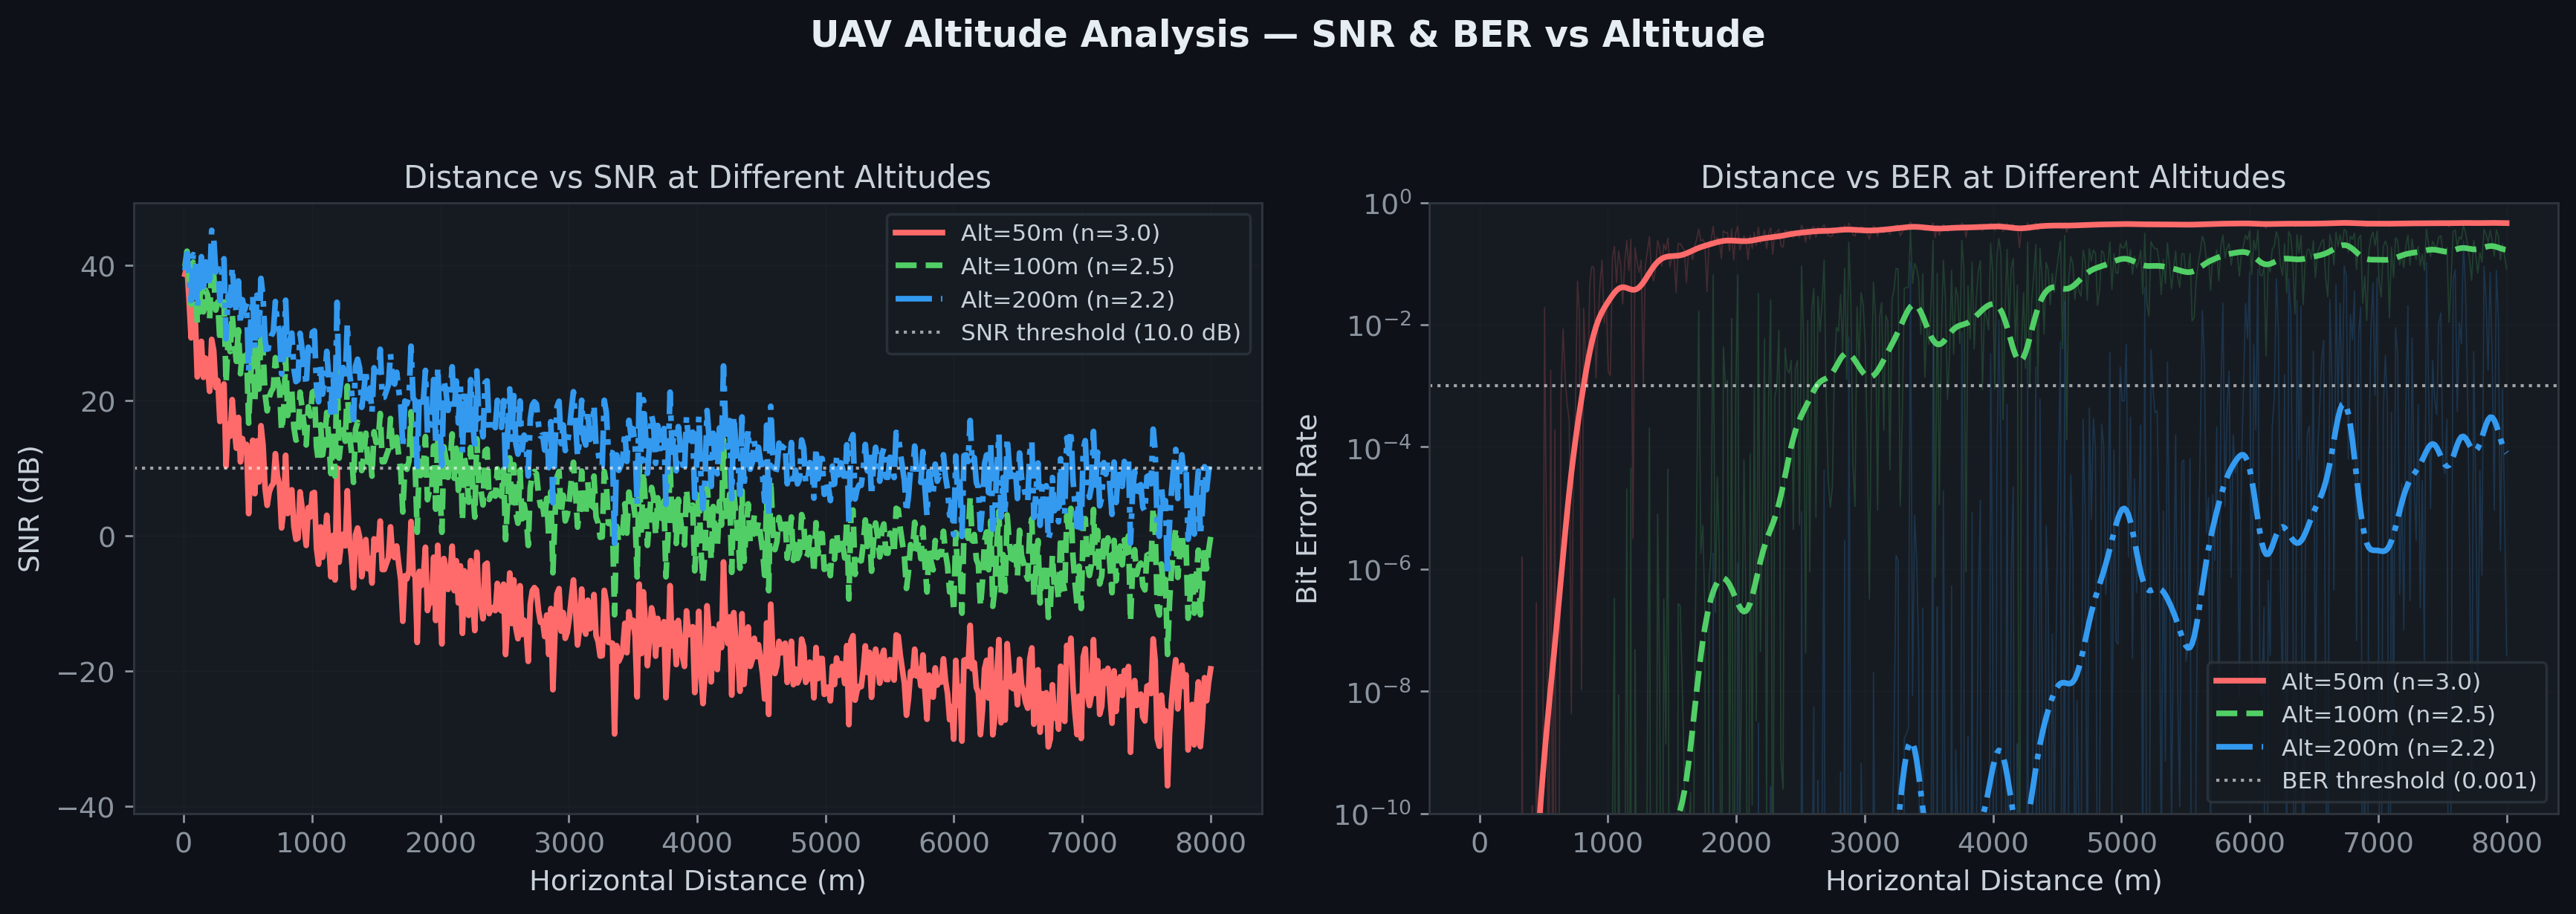
\includegraphics[width=\textwidth]{fig9_altitude_analysis.png}
\caption{\footnotesize Altitude analysis: range vs.\ UAV altitude with altitude-dependent path-loss exponents.}
\end{figure}
\end{column}
\end{columns}
\end{frame}

% ============================================================
% E. CONCLUSION
% ============================================================
\section{Conclusion}

\begin{frame}{Conclusion}
\begin{block}{Key Achievements}
\begin{itemize}
  \item Combined techniques extend baseline range from \textbf{4,573\,m to 8,000\,m} (+74.9\%).
  \item GA-based power control achieves \textbf{7,952\,m} with \textbf{55.7\% less energy} (248.1 vs.\ 560.7\,mW).
  \item Formal EE metric confirms GA superiority: \textbf{32.1 vs.\ 14.3\,m/mW}.
  \item Rician fading ($K\!=\!6$) maintains stable baseline performance for LoS-dominant UAV channels.
  \item Altitude optimisation yields \textbf{6.7$\times$} range improvement (50\,m $\to$ 200\,m).
  \item Three-tier adaptive modulation provides \textbf{33\% higher near-field throughput}.
\end{itemize}
\end{block}

\vspace{0.3cm}

\begin{exampleblock}{Future Work}
\begin{itemize}
  \item Joint trajectory--power optimisation using multi-objective evolutionary algorithms.
  \item Multi-UAV cooperative communication for extended coverage.
  \item Hardware-in-the-loop validation with real UAV platforms.
\end{itemize}
\end{exampleblock}
\end{frame}

% ── References ───────────────────────────────────────────────
\section{References}

\begin{frame}{References}
\footnotesize
\begin{thebibliography}{11}
\bibitem{b0} L.~Uryvsky et al., ``Improving the distance-extension methods for reliable wireless communication in IoT networks with UAV,'' \textit{Proc. IEEE TCSET}, 2024.
\bibitem{b1} A.~Al-Fuqaha et al., ``Internet of things: A survey,'' \textit{IEEE Commun. Surveys Tuts.}, 2015.
\bibitem{b2} Y.~Zeng et al., ``Wireless communications with UAVs,'' \textit{IEEE Commun. Mag.}, 2016.
\bibitem{b3} A.~Al-Hourani et al., ``Optimal LAP altitude for maximum coverage,'' \textit{IEEE Wireless Commun. Lett.}, 2014.
\bibitem{b5} T.~S.~Rappaport, \textit{Wireless Communications}, 2nd ed., Prentice Hall, 2002.
\bibitem{b7} M.~Mozaffari et al., ``Efficient deployment of multiple UAVs,'' \textit{IEEE Commun. Lett.}, 2016.
\bibitem{b8} J.~G.~Proakis and M.~Salehi, \textit{Digital Communications}, 5th ed., McGraw-Hill, 2008.
\bibitem{b11} M.~K.~Simon and M.-S.~Alouini, \textit{Digital Communication over Fading Channels}, 2nd ed., Wiley, 2005.
\end{thebibliography}
\end{frame}

% ────────────────────────────────────────────────────────────
% THANK YOU
% ────────────────────────────────────────────────────────────
{
\setbeamertemplate{footline}{}
\begin{frame}[plain]
\vfill
\centering
{\Huge\textcolor{iiitblue}{\textbf{Thank You!}}}

\vspace{0.8cm}
{\large Questions \& Discussion}

\vspace{1cm}
\begin{tabular}{rl}
\textcolor{iiitblue}{\textbf{Email:}} & \texttt{palvashkumar.a23@iiits.in} \\[4pt]
                                       & \texttt{mood.n23@iiits.in} \\[8pt]
\textcolor{iiitblue}{\textbf{GitHub:}} & \href{https://github.com/Palvash-kumar/IOT_team-paper}{\texttt{github.com/Palvash-kumar/IOT\_team-paper}} \\
\end{tabular}
\vfill
\end{frame}
}

\end{document}
